% Chapter containing details about the hysteresis of the muscle
% Outline:
% - Introduction
% - Evolutionary algorithms outline
%	- Genetic Algorithm
% - Multi-variable optimization
% 	- Firefly Algorithm
% 	- Modified Firefly Algorithm
% 	- PSO
% - Implementation
% - Results comparison

\chapter{Hysteresis Parameter Optimization}
\label{ch:optimization}

In this chapter, the methods to obtain the model's parameters are explained.
As shown in Section~\ref{sec:4.eva}, although parameters cherry-picked by trial
and error proved successful to fit the approximated model onto experimental data,
a higher grade of precision is desirable for applications demanding high accuracy.

Section~\ref{sec:5.evo} introduces the concept of \textit{evolutionary algorithm},
with particular regard towards a simple genetic algorithm approach
with the purpose of optimization.

After that, Section~\ref{sec:5.opt} introduces methods of \textit{metaheuristic
algorithm}, with the goal of transforming the search of parameters
into an optimization problem.

Section~\ref{sec:5.res} contains results and comparison
for all algorithms previously described.


\section{Introduction}
After having described how to get a discrete model of the McKibben artificial muscle,
the Bouc-Wen model of hysteresis has been introduced.
This model proves useful to describe a hysteretic behaviour in a simple manner,
and can provide great advantages in terms of performance when it comes to control.

However, there are parameters that have to be tuned in order for the model
to operate correctly. The tuning may be done by trial and error, or the whole process
may be automated.

The parameter refinement process makes use of an algorithm to
find the parameters of the Bouc-Wen model that give a best approximation
of the real experimental data. Such algorithms include, but are not limited to,
Recursive Least Squares (RLS), evolutionary algorithms
and multi-variable optimization algorithms.

For this work, different approaches based on evolutionary algorithms
and multi-variable optimization methods have been tested.

%\clearpage

\section{Evolutionary Algorithms}
\label{sec:5.evo}

An evolutionary algorithm is a population-based optimization algorithm
that mimics the behaviour of biological evolution, simulating the steps of
reproduction, mutation, recombination and selection.

Each individual is tested in an optimization problem,
and the best characteristic of the population are passed through the generations.
The evaluation of an individual is done by means of a fitness function.
A fitness function is a operator that assigns a fitness value to each individual.
Depending on the nature of the problem, individuals with lower (or higher)
fitness values are judged "better" from the algorithm and have a higher probability
of being chosen in the mating step to generate new, better individuals.
Therefore, their characteristics have a higher chance to be passed onto next generations
in order to iteratively refine the parameters and arrive at a acceptable solution.

After a certain amount of generations, or after one individual reaches
a fixed fit value, the algorithm stops and the best individual is chosen
as the solution to the optimization problem.

\subsection{Genetic Algorithm}
\label{sec:5.ga}

A genetic algorithm (GA)~\cite{fleming2001genetic} is a kind of evolutionary algorithm inspired
by the concept of natural selection that permeates a biological evolutionary process.

Genetic algorithms are a class of stochastic global search algorithm
operating on a set called \textit{population} of current approximations,
called \textit{individuals}.
Individuals are encoded as a set (\textit{chromosome}) of parameters (\textit{genes}).

Once a population has been created, each individual performance is assessed
according to the objective function characterising the problem that has to be solved.

Algorithms belonging to this class are divided into the following steps:
\textit{initialization}, \textit{evaluation}, \textit{crossover} and \textit{mutation}.
The general outline of the procedure is shown in Algorithm~\ref{alg:ga}.
The description and peculiarities of each step are discussed in Section~\ref{sec:5.steps}.
The genetic algorithm also makes use of several parameters, which are summarized
in Table~\ref{tab:ga_params}.

\begin{table}[]
	\centering
	\begin{tabularx}{\linewidth}{c X}
		\toprule
		\textbf{Parameter} & \textbf{Description} \\ \midrule
		$N$        & The population's size, i.e. the number of individuals (candidate solutions) that evolve to find a good approximation. \\
		$G$         & The maximum generation. After reaching that stage of evolution, the algorithm stops. \\
		$d$           	   & The chromosome's dimension, i.e. the number of variables to be optimized by the algorithm. \\
		$L$           	   & A $d$-dimensional vector containing the lower bounds for each variable. \\
		$U$				   & A $d$-dimensional vector containing the upper bounds for each variable. \\
		$P_{cross}$		   & The crossover probability. It controls the chance of inheriting a chromosome from a specific parent with respect to the other. \\
		$P_{mut}$		   & The mutation probability. \\
		$m_m$			   & The mutation magnitude, i.e. how much a given chromosome changes in the event of a mutation. \\ \bottomrule
	\end{tabularx}
	\caption{Parameters for the genetic algorithm}
	\label{tab:ga_params}
\end{table}

\subsubsection{Algorithm Overview}

\begin{algorithm}
	\caption{Genetic algorithm approach} \label{alg:ga}
	\begin{algorithmic}
		\Procedure{Genetic Algorithm}{}\newline
		\textbf{Input:} $N$, $G$, $d$, $L$, $U$, $p_{cross}$, $p_{mut}$, $m_m$\newline
		\textbf{Output:} \textit{A $d$-dimensional vector, i.e. the candidate solution (individual) with best fit value}
		\State{\textbf{Initialization:} \textit{generate $N$ $d$-dimensional vectors} $n_i, i \in \left[1,N\right]$}
		\State{$current\_gen \gets 1$}
		\While{$current\_gen < G$}
			\State{\textbf{Evaluation:} \textit{compute the fit value $fit(i)$ for each vector}}
			\State{\textit{Compute the normalized fit value $fit_n(i)$ for each vector}}
			\State{$M_p \gets$ \textit{new empty Set}}
			\While{$\lvert \mathcal M_p \rvert<N$}
				\State{\textbf{Crossover:} \textit{extract 2 individuals}}
				\State{\textit{Generate 2 new individuals (offspring)}}
				\State{\textit{Add the offspring to} $M_P$}
			\EndWhile{\textbf{end while}}
			\State{\textbf{Mutation:}}
			\ForEach{$m \in \mathcal M_p$ }
				\ForEach{\textit{gene} $m_i, i=1,\ldots,d$}
					\State{\textit{Generate a random value $r$ such that} $0\le r \le 1$}
					\If{$r\le P_{mut}$}
						\State{\textit{Mutate the i-th gene with percentage} $\pm m_m\%$}
					\EndIf
				\EndFor
			\EndFor
		\EndWhile{\textbf{end while}}
		\State{\textit{Return the individual with best fit value}}
		\EndProcedure
	\end{algorithmic}	
\end{algorithm}

\subsubsection{Algorithm Description}


\label{sec:5.steps}
\subsubsection{Initialization Step}

For a genetic algorithm, the initialization step consists in the creation
of the individuals, and by extension that of the population.

One of the most common initialization methods is random initialization:
each gene of any individual is randomly chosen between a defined interval.
This gives a higher chance of finding good results from the first generations,
and refine the solution starting from them.

Another initialization method may be to create a population of equal
individuals, and mainly rely on mutation for the first generations
in order to find better approximations. This method, while it may better
reflect the natural behaviour of a biological evolutionary process,
takes also a much larger number of generations to return appreciable results.

For this reason, the GA developed for this work makes use of random initialization.
$N$ $d$-dimensional vectors (individuals) $p$ are created,
following the constraints in Equation~\ref{eq:constraints}.

\begin{align}
\begin{cases}
	p_i = \left[p_{i1},\ldots,p_{id}\right] \\
	L_j \leq p_{ij} \leq U_j, \quad i=1,\ldots,N, \quad j=1,\ldots,d
\end{cases}
\label{eq:constraints}
\end{align}


\subsubsection{Evaluation Step}

The evaluation step concerns assessing a fitness value to each individual
in order to rank them according to their performance in solving the optimization problem.
The fitness value is assigned to each individual by means of a \textit{fitness function}.

Experimental input pressure and output displacement,
respectively described in Equations~\ref{eq:exp_pres} and~\ref{eq:exp_disp},
are taken from data acquired by the identification experiments described
in Section~\ref{sec:4.ide}. 

\begin{align}
u &= \left[u_1,u_2,\ldots,u_k\right] \label{eq:exp_pres} \\
l &= \left[l_1,l_2,\ldots,l_k\right] \label{eq:exp_disp}
\end{align}

with $k$ representing the number of points for which the experimental data
has been sampled.

Each individual is used to perform a specific simulation of the model with its genes
set as Bouc-Wen hysteresis parameters, using $u$ as input.
The simulated output displacement $\hat{l}$
is then compared to the experimental displacement $l$.

The fitness function chosen for this step is described in Equation~\ref{eq:fitness}.
This function returns the fitness value for the i-th individual of the population.

\begin{align}
fit(i) = \frac{1}{\sum_{i=1}^k{\left(l_i-\hat{l}_i\right)^2}}
\label{eq:fitness}
\end{align}

Judging from the nature of the fitness function, it is clear that
individuals with a fitness value close to 0 are better than others,
as it means that their simulated output is close to experimental data.

After that, the fit value of each individual is normalized in order to be used
for the crossover step. To do so, each fit value is divided by the sum of all fit values,
as shown in Equation~\ref{eq:fit_norm}.

\begin{align}
fit_n(i) = \frac{fit(i)}{\sum_{i=1}^n fit(i)}
\label{eq:fit_norm}
\end{align}

It is important to notice that given the way that $fit_n$ is constructed,
the relation of Equation~\ref{eq:sum_1} arises.

\begin{align}
\sum_{i=1}^N fit_n(i) = 1
\label{eq:sum_1}
\end{align}

\subsubsection{Crossover Step}

The crossover step serves the purpose of creating two new individuals (\textit{offspring})
starting from two \textit{parents}. The characteristics of the offspring will thus
largely depend on their parents' ones.

Three different crossover policies have been developed for this purpose:


\begin{itemize}[noitemsep]
	\item \textbf{Random crossover}
	
	The random method assigns the genes from parents to offspring in a random fashion.
	
	Given a number $x$ with $1 \le x \le d$,
	the offspring inherits the first $x$ genes from the first parent and
	the remaining ones from the second parent.
	This process is repeated for the second offspring.
	\item \textbf{Weighted crossover}
	
	The weighted method makes so that the genes of the parent with higher
	fit have a higher probability of being chosen for the offspring.
	
	Given the fit values of the parents $fit(p_1)$ and $fit(p_2)$,
	with $fit(p_1) \ge fit(p_2)$, then the \textit{inheritance probability} $In_p$
	is defined as follows:
	
	\begin{align*}
	In_p = \frac{fit(p_1)}{fit(p_1)+fit(p_2)}
	\end{align*}
	
	For each offspring and gene, the probability of inheriting the given gene
	from the first parent will be $In_p$. Otherwise, the gene will be inherited
	from the second parent.
	\item \textbf{Proportional crossover}
	
	The proportional method creates the offspring's genes from the parents' ones,
	proportionally inheriting them based on their fit values.
	
	Given the fit values of the parents $fit(p_1)$ and $fit(p_2)$,
	with $fit(p_1) \ge fit(p_2)$, then the \textit{proportion variables} $pv_1$
	and $pv_2$ are defined as follows:
		
	\begin{align*}
	pv_1 = \frac{fit(p_1)}{fit(p_1)+fit(p_2)},\quad pv_2 = 1-pv_1
	\end{align*}
	
	Given $Gp_1(x), Gp_2(x), Go(x), 1\le x\le d$
	respectively for the first parent's, the second parent's
	and the offspring's	$x$-th gene, then the following relation arises:
	
	\begin{align*}
		Go(x) = Gp_1(x)\cdot pv_1 + Gp_2(x) \cdot pv_2
	\end{align*}

	This means that the offspring will be more similar
	to the parent with higher fit, while still carrying on some of 
	the less performing parent's characteristics.
\end{itemize}


\subsubsection{Mutation Step}

The mutation step's purpose is to randomly mutate some genes to reflect
the random behaviour of biological evolution through time. 

For each gene $Go(x), 1\le x \le d$ of each offspring generated,
a random value $r$ between $0$ and $1$ is generated. If this value
is less than the \textit{mutation probability} $P_{mut}$, then
the gene is modified by a percentage of its value.

The final value $Go(x)'$ of the x-th gene will be:

\begin{align*}
Go(x)' = Go(x)\cdot \left(1 \pm m_m\right)
\end{align*}

Here the \textit{mutation magnitude} is added or subtracted
with probability $0.5$, by generating a new random value and
verifying whether it surpasses this threshold.

\section{Metaheuristic Algorithms}
\label{sec:5.opt}

A \textit{metaheuristic} is a procedure designed to find a heuristic
that may provide a sufficiently good solution to an optimization problem.

Metaheuristic algorithms do not guarantee that a globally optimal solution
can be found on some class of problems, but they often provide a solution
with a good fit value by exploring the space of possible solutions.

For this work, two metaheuristic algorithms have been developed and tested
with the purpose of finding good parameters for fitting the Bouc-Wen hysteresis
parameters of the identified transfer function over real experimental data.

The first is the \textit{Firefly Algorithm}, described in Subsection~\ref{sec:5.fa}.
This algorithm mimics the movement of a swarm of fireflies inside the solution space,
simulating an \textit{attractiveness component}, governed by their \textit{luminosity},
that pushes the swarm towards local and global optimal solutions.
Two versions of this algorithm have been developed in order to grant a higher
versatility for finding the parameters, depending on the required application.
The modified version is described thoroughly in Section~\ref{sec:5.mfa}.

The second algorithm is the \textit{Particle Swarm Optimization},
described in Section~\ref{sec:5.pso}. It is a computational method that optimizes a
problem by iteratively trying to improve a candidate solution with regard to a given
measure of quality. It solves a problem by having a population of candidate solutions
(\textit{particles}) moving around in the search-space according to simple laws
governed by their position and velocity.
Each particle's movement is influenced by its local best known position,
but is also guided toward the best known positions in the search-space.
This value is updated whenever a better position is found any particle.
This is expected to move the swarm toward the best solutions.
The algorithm has been conceived as a mathematical representation
of the movement of organisms in a bird flock or fish school.

The values chosen for algorithms' parameters are discussed in Section~\ref{sec:5.res},
which is dedicated to show the results and compare these algorithms.


\subsection{Firefly Algorithm}
\label{sec:5.fa}

The Firefly Algorithm (FA) is a metaheuristic optimization algorithm
developed by Xin-She Yang~\cite{yang2010nature} that mimics the behaviour
of fireflies.

The main concept of such algorithm is to create a population of fireflies
representing candidate solutions in a $d$-dimensional space 
for a certain optimization problem, where $d$ is the number of variables to be optimized.

The fireflies are then attracted to each other following a set of rules:

\begin{itemize}[noitemsep]
	\item \textbf{Unisexuality} 
	
	All fireflies are unisex, so that one firefly is attracted
	to other fireflies regardless of their sex.
	\item \textbf{Attractiveness}
	
	The attractiveness of a firefly is proportional to its brightness,
	thus for any two fireflies the less bright will move towards the brighter one.
	Both brightness and attractiveness decrease as the distance between
	two fireflies increases.
	\item \textbf{Brightness}
	
	The brightness of a firefly is determined and affected by the objective function.
\end{itemize}


\subsubsection{Algorithm Overview}

\begin{algorithm}
	\caption{Firefly Algorithm Approach} \label{alg:fa}
	\begin{algorithmic}
		\Procedure{Firefly Algorithm}{}\newline
		\textbf{Input:} $N$, $G$, $d$, $L$, $U$ \newline
		\textbf{Output:} \textit{A $d$-dimensional vector,
			i.e. the candidate solution (firefly) with best fit value}
		\State{\textbf{Initialization:} \textit{generate $N$ $d$-dimensional vectors} $n_i, i \in \left[1,N\right]$}
		\State{\textit{Light intensity} $I_i$ for $n_i$
			\textit{is determined by} $\mathit{f}(n_i)$}
		\State{\textit{Define light absorption coefficient $\sigma$}}
		\State{$current\_gen \gets 1$}
		\While{$current\_gen < G$}
			\For{$i = 1,\ldots,N$}
				\For{$j = 1,\ldots,N$}
					\If{$I_i < I_j$}
						\State{\textit{Move firefly i towards j}}
						\EndIf
					\State{\textit{Vary attractiveness with distance} $r$}
					\State{\textit{Evaluate new solutions and update light intensity}}
				\EndFor
				\State{\textbf{end for} $j$}
			\EndFor
			\State{\textbf{end for} $i$}
			\State{\textit{Rank the fireflies and find the current global best $g^*$}}
		\EndWhile
		\State{\textbf{end while}}
		\EndProcedure
	\end{algorithmic}
\end{algorithm}

\subsubsection{Algorithm Description}

The following sections serves the purpose of describing in depth the steps
and the specifics of the Firefly Algorithm.

Section~\ref{sec:5.light_attract} describes how light intensity influences
the relative attractiveness between two fireflies. 

Section~\ref{sec:5.famovement} describes how fireflies move in the solution
space through the iterations.

Table~\ref{tab:fa_params} summarizes and describes the parameters used by the algorithm.

\begin{table}[]
	\centering
	\begin{tabularx}{\linewidth}{c X}
		\toprule
		\textbf{Parameter} & \textbf{Description} \\ \midrule
		$N$        & The population's size, i.e. the number of fireflies (candidate solutions) that move in the solution space to find a good solution. \\
		$G$         & The maximum generation. After reaching that stage of evolution, the algorithm stops. \\
		$d$           	   & The chromosome's dimension, i.e. the number of variables to be optimized by the algorithm. \\
		$L$           	   & A $d$-dimensional vector containing the lower bounds for each variable. \\
		$U$				   & A $d$-dimensional vector containing the upper bounds for each variable. \\ 
		$\Lambda_0$ & Attractiveness at zero distance, described in Section~\ref{sec:5.azd} \\
		$\sigma$		& Light absorption coefficient that influences the attractiveness distance, described in Section~\ref{sec:5.lac}. \\
		$\rho$ & Randomization parameter influencing the fireflies' motion, described in Section~\ref{sec:5.rp} \\ \bottomrule
	\end{tabularx}
	\caption{Parameters for the genetic algorithm}
	\label{tab:fa_params}
\end{table}

\subsubsection{Light Intensity and Attractiveness}
\label{sec:5.light_attract}

The brightness $I$ of a firefly at a particular location depends
on the fitness value returned by the fitness function at that specific location.

Each firefly follows a path that brings it closer to other
attractive fireflies. Relative attractiveness $\Lambda_{ij}$ however is relative,
and it will vary with the distance $r_{ij}$ between firefly \textit{i} and \textit{j}.

Equation~\ref{eq:attractiveness} shows the relation between distance and attractiveness,
where $\Lambda_0$ is the attractiveness at zero distance and $\sigma$ is
a parameter called \textit{light absorption coefficient}.

\begin{align}
\label{eq:attractiveness}
\Lambda_{ij}=
\begin{cases}
\Lambda_0 e^{-\sigma r_{ij}^2} & \text{if } I_j > I_i \\
0 & \text{otherwise}
\end{cases}
\end{align}

Equation~\ref{eq:attractiveness} suggests that the brighter is a firefly,
the more attractive it is to any other firefly. The light intensity $I_j$
for the \textit{j}-th firefly is determined by the fit function.

\begin{align}
I_j = \mathit{f}_{fit}(n_j) = \mathit{f}_{fit}(n_{j,1},n_{j,2},\ldots,n_{j,d})
\end{align}


The fit function chosen for this work is the same as for the Genetic Algorithm
approach, and is shown in Equation~\ref{eq:fitness}. 
The distance $r_{ij}$ between firefly \textit{i} and \textit{j}
at step \textit{k} is given by the Euclidean distance between the two.

\begin{equation}
\begin{cases}
r_{ij}^k &= \norm{n_j^k-n_i^k} \\ 
&= \sqrt{(n_{j,1}^k-n_{i,1}^k)^2+(n_{j,2}^k-n_{i,2}^k)^2+\ldots+(n_{j,d}^k-n_{i,d}^k)^2}
\end{cases}
\end{equation}

\subsubsection{Firefly Movement}
\label{sec:5.famovement}

The movement of a firefly $n_i$ towards a more attractive $n_j$ 
at step $k \in \left[1,G\right]$ is given by Equation~\ref{eq:fa_movement}.

\begin{align}
\label{eq:fa_movement}
n_i^k = n_i^k + \Lambda_{ij}^k\left(n_j^k-n_i^k\right)+\rho \mathit{v}_i^k
\end{align}

Here $\Lambda_{ij}$ is the attractiveness of firefly \textit{j} to firefly \textit{i},
$\rho$ is a \textit{randomization parameter} and $\mathit{v}_i$ is
a vector of $d$ random numbers drawn from a Gaussian or uniform distribution.

It is important to notice that the movement of a given firefly
towards a less attractive one is given only by a random factor, but it is still present.
This means that the most attractive fireflies still move and can
potentially find better solutions.

After the fireflies' positions are updated, new fitness values
are calculated. New generations are obtained
by using the same set of equations. Over successive generations,
the fireflies converge to local and global optimal values,
completing the optimization process.


\subsection{Modified Firefly Algorithm}
\label{sec:5.mfa}

A modified version of the Firefly Algorithm has been developed and studied
by M.A. Zaman and U. Sikder~\cite{zaman2015bouc}. The main idea behind
the Modified Firefly Algorithm is to change the \textit{process control parameters}
$\Lambda_0$, $\sigma$ and $\rho$ through the iterations. Typical values
of these parameters are $\Lambda_0=1$, $\sigma = 1$ and $\rho \in \left[0.1,0.2\right]$.
By changing these from static to dynamic parameters it is possible to perform
a more precise tuning of the fireflies behaviour, reflecting thus on the performance
of the algorithm on finding their optimal values.

\subsubsection{Attractiveness at Zero Distance}
\label{sec:5.azd}

It has been studied that the attractiveness at zero distance parameter $\Lambda_0$
controls the \textit{exploration distance} of the fireflies: 
higher values of $\Lambda_0$ encourage global exploration while
lower values encourage close refinement (local exploitation). 

Hence it would be better to make $\Lambda_0$ a decreasing value over the iterations, 
such that initially the fireflies explore a wide range of possible solutions
minimizing the risk of getting stuck in a local optimum, while 
near the end of the execution a lower value would allow for fine refinement
around the different optima found.

The formula for the attractiveness parameter for iteration
$k\in \left[1,G\right]$ has been changed as shown in Equation~\ref{eq:attr_changed}.

\begin{align}
\label{eq:attr_changed}
\Lambda_0(k) = a - b\frac{1-k}{1-G}
\end{align}

From Equation~\ref{eq:attr_changed} it is possible to notice
that the value of $\Lambda_0$ goes from $a$ (when $k=1$) to $a-b$ (when $k=G$).

\subsubsection{Light Absorption Coefficient}
\label{sec:5.lac}

The value of $\sigma$ control the effect of distance on the motion of fireflies.
Equation~\ref{eq:attractiveness} suggests that lower values of $\sigma$ will
cause movement towards other attractive fireflies even if they are far away.
This may lead to a premature convergence of a high number of fireflies
towards a local maximum.

However, after a sufficient number of generations, it is desirable
that the fireflies start to converge towards the maximum value found so far.
To do so, a lower value of $\sigma$ is required.

The formula for the \textit{light absorption coefficient} $\sigma$
for iteration $k$ has been changed as shown in Equation~\ref{eq:lac_changed}.

\begin{align}
\label{eq:lac_changed}
\sigma(k) = 2 \cdot \left(7^{\nicefrac{-k}{G}}\right),\quad c \ge 0, d \ge 0
\end{align}

\subsubsection{Randomization Parameter}
\label{sec:5.rp}

The \textit{randomization parameter} $\rho$ controls the random component
of the firefly's motion. A large value of $\rho$ encourages broad random exploration.
Using the same arguments as for the \textit{light absorption coefficient},
it can be inferred that a gradual decrease of the value of $\rho$ over
successive iterations should improve the performance of the algorithm
as the fireflies must explore the solution space widely at the beginning
to find good candidate solutions and then refine them in latter steps.

The formula for the \textit{randomization parameter} $\rho$
for iteration $k$ has been changed as shown in Equation~\ref{eq:random_changed}.

\begin{align}
\label{eq:random_changed}
\rho(k) = 0.1 \cdot e^{\nicefrac{-4.8k}{G}}
\end{align}

The proposed modification of the algorithm using dynamic parameters
are expected to provide a good mix of global exploration and local exploitation,
resulting in high accuracy and fast convergence of the algorithm towards
the global optimum.

\subsection{Particle Swarm Optimization}
\label{sec:5.pso}

Particle Swarm Optimization (PSO) is an evolutionary computation technique
developed by Kennedy and Eberhart in 1995~\cite{kennedy2011particle}~\cite{eberhart1995new}.

PSO is similar to a genetic algorithm, meaning that both algorithms 
are initialized with a population of random solutions. Unlike a GA, however,
candidate solutions, called \textit{particles}, are also assigned a randomized velocity.
After that, they are flown into the problem space.

Each point of the problem space represents a set of parameters for the optimization
problem that has to be solved, in this case the Bouc-Wen model parameter search
Each particle keeps track of its coordinates in the problem space,
and remembers the coordinate of the point which has yielded the best solution,
in other words the point that has the highest fitness value found by them so far.
This value is called \textit{pbest}, which means \textit{personal best}.

Another value is tracked and known by all particles, which is the \textit{global best}
value found by any particle up until that certain iteration of the algorithm.
This value is called \textit{gbest}.

The particle swarm optimization concept consists of, at each time step,
changing the velocity (accelerating) each particle towards its \textit{pbest}
and \textit{gbest} locations. Acceleration is weighted by a random term,
with separate random numbers generated to dictate acceleration towards
\textit{pbest} and \textit{gebest} locations.

\subsubsection{Algorithm Overview}

\begin{algorithm}[H]
	\caption{Particle swarm optimization approach} \label{alg:pso}
	\begin{algorithmic}
		\Procedure{Particle Swarm Optimization}{}\newline
			\textbf{Input:} $N$, $G$, $d$, $L$, $U$, $V_{max}$\newline
			\textbf{Output:} \textit{A $d$-dimensional vector, i.e. the candidate solution (particle) with best fit value}
			\State{\textbf{Initialization:} \textit{generate $N$ $d$-dimensional vectors} $n_i, i \in \left[1,N\right]$}
			\State{$current\_gen \gets 1$}
			\While{$current\_gen < G$}
				\State{\textbf{Evaluation:} \textit{compute the fit value $fit(i)$ for each vector}}
				\State \begin{varwidth}[t]{.85\textwidth} 
					\textbf{Pbest comparison:} \textit{Compare the particle's fit value with particle's $pbest$.
						If the current value is better than $pbest$, then set $pbest$ value equal to the current value, and $pbest$ location equal to the particle's current location in the $d$-dimensional space}
					\end{varwidth}
				\State \begin{varwidth}[t]{.85\textwidth} 
					\textbf{Gbest comparison:} \textit{Compare the particle's fit value with $gbest$.
						If the current value is better than $gbest$, then set $gbest$ value equal to the current value, and $gbest$ location equal to the particle's current location in the $d$-dimensional space}
					\end{varwidth}
				\State \textbf{Update:} \textit{change the particle's velocity and position}
			\EndWhile{\textbf{end while}}
		\EndProcedure
	\end{algorithmic}
\end{algorithm}

\subsubsection{Algorithm Description}

The following sections serve the purpose of describing in depth the steps
and the specifics of the Particle Swarm Optimization algorithm.

Section~\ref{sec:5.pso.speed} describes how the values for velocity and position
for the particles are updated each iteration.

Section~\ref{sec:5.inertia} describes the purpose of and how to compute
the inertia weight $w$ used when calculating the speed of a particle.

Section~\ref{sec:5.pso.constants} describes the purpose of the acceleration
constants $c_1$ and $c_2$.

\subsubsection{Velocity and Position Update}
\label{sec:5.pso.speed}

Given $x_i$ and $v_i$ which are respectively the \textit{i}-th particle's position
and velocity, then the movement of the \textit{i}-th particle is dictated by
Equations~\ref{eq:pso_velocity} and~\ref{eq:pso_position}.
In Equation~\ref{eq:pso_velocity}, $w$ is the \textit{inertia weight},
$x_{pb}$ is the position associated to the particle's personal best value, 
and $x_{gb}$ is the position associated to the global best value among all particles.

\begin{align}
v_i &= w\cdot v_i + c_1 \cdot rand() \left(x_{pb}-x_i\right)+c_2\cdot rand() \left(x_{gb}-x_i\right) \label{eq:pso_velocity} \\
x_i &= x_i + v_i \label{eq:pso_position}
\end{align}

Particles' velocity are constrained by the maximum velocity parameter $V_{max}$.
This is a very important parameter, as it determines the fineness with which regions
between the present position and the best positions known are searched.
If $V_{max}$ is too high, particles my overshoot good solutions. On the other hand,
if $V_{max}$ is too low, particles may move very slowly and may not be able to find
a good solution before the algorithm comes to a halt.

\subsubsection{Inertia Weight}
\label{sec:5.inertia}

The use of a \textit{inertia weight} $w$ has provided improved performance
in a number of applications, as an opportune selection of the inertia weight 
provides a balance between global and local exploration,
and results in fewer iterations on average to find a sufficiently good solution.

The \textit{inertia weight} w changes dynamically with the current iteration
of the algorithm according to the following law:

\begin{align*}
	w(k) = a-(a-b)\cdot \frac{k}{G},\quad k \in \left[1,G\right]
\end{align*}

\subsubsection{Acceleration Constants}
\label{sec:5.pso.constants}

The \textit{acceleration constants} $c_1$ and $c_2$ represent
the importance of the personal and global best according to the particles.
If $c_1$ is greater than $c_2$, the particles will tend to judge as better
their own personal best and will be inclined to move towards that location.


\section{Algorithm Comparison}
\label{sec:5.res}

Simulations have been run on all the algorithms proposed in the previous sections.
Each one of them has been tested with both the standard and the generalized Bouc-Wen
model of hysteresis. The results, for both models and for each algorithm,
are respectively in Section~\ref{sec:5.comp_res_classic} and~\ref{sec:5.comp_res_gen}.

Since the generalized version of the hysteresis component consists of 8 variables
it is safe to assume beforehand that the execution time of the algorithms would be higher.
A comprehensive comparison of the execution times for the algorithms is described in
Section~\ref{sec:5.comparison_time}.



\subsection{System Specifications}

%TODO scrivere le system specifications del pc

\subsection{Solution Comparison -- Classic Bouc-Wen Model}
\label{sec:5.comp_res_classic}

This Section serves the purpose of comparing the solutions found using the
algorithms previously described when trying to find suitable parameters
for the classic Bouc-Wen model of hysteresis.

\subsubsection{Genetic Algorithm -- Classic Bouc-Wen Model}

Table~\ref{tab:ga_classic_params} contains the parameters used
for the genetic algorithm approach. Those parameters have been used for
the genetic algorithm using all three kinds of crossover strategies:
random, weighted and proportional.

Figures~\ref{fig:ga_classic_rand},~\ref{fig:ga_classic_w}
and~\ref{fig:ga_classic_prop} show the trend of the classic Bouc-Wen model
parameters $A$, $\alpha$, $\beta$ and $\gamma$ depending on the
crossover strategy used~\footnote{Figure~\ref{fig:ga_classic_rand} shows, for each generation,
the parameters of the best individual, i.e. the individual with the highest fit value.
This will be the standard way of presenting trends from now on.}.

It is important to note that due to how the three strategies have been developed,
the performance of the random and weighted methods depend strictly on
the initial population, as the individuals' chromosomes are always only swapped.
The final result will approach the best possible solution attainable
using the chromosomes of the initial population~\footnote{
	Apart from eventual changes introduced in case of mutations.}. 
However, it is certainly possible that the final fit may not be acceptable.

Due to this fact, the proportional crossover strategy proved to be the best
as it generates new chromosomes (and thus, completely new individuals)
each generation. Regardless, a decreasing trend in each parameter is to be expected
due to how the proportional strategy has been developed.

\begin{table}[]
	\centering
	\begin{tabular}{c c}
		\toprule
		\textbf{Parameter} & \textbf{Value} \\ \toprule
		$N$			& $30$ \\
		$G$			& $30$ \\
		$d$			& $4$  \\
		$L$			& $\left[0.5, 0.5, -0.5, -0.1\right]$ \\
		$U$			& $\left[1, 0.99, 0.5, 0.1\right]$ \\ 
		$P_{cross}$	& $0.5$ \\
		$P{mut}$	& $0.1$ \\
		$m_m$		& $0.05$ \\	\bottomrule
	\end{tabular}
	\caption{Parameters for the Genetic Algorithm approach -- Classic Bouc-Wen model}
	\label{tab:ga_classic_params}
\end{table}


\begin{figure}[H]
	\centering
	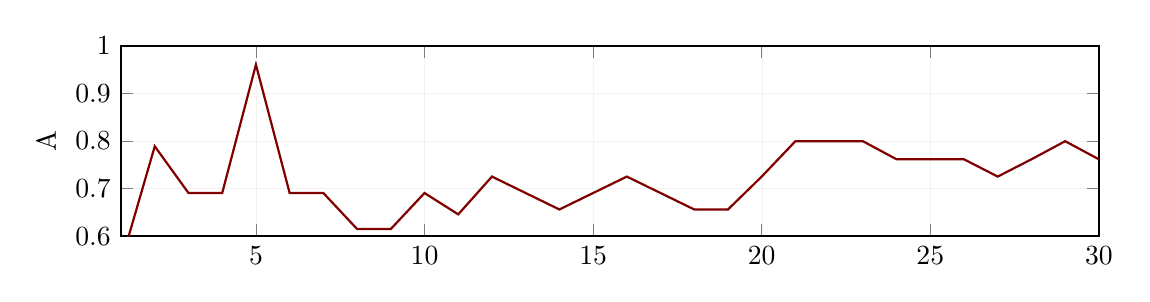
\begin{tikzpicture}
	\begin{axis}[
	%	xlabel={Generation},
	ylabel={A},
	xmin=1, xmax=30,
	ymin=0.6, ymax=1,
	grid=both,
	grid style={line width=.1pt, draw=gray!10},
	width=14cm,height=4cm,
	xtick={0,5,10,15,20,25,30},
	ytick={0.6,0.7,0.8,0.9,1},
	thick]
	
	\addplot[color=Maroon]
	coordinates {
		(1,0.545135339844412)(2,0.788923360170356)(3,0.690777924711849)
		(4,0.690777924711849)(5,0.960441630068157)(6,0.690777924711849)
		(7,0.690777924711849)(8,0.615202221951477)(9,0.615202221951477)
		(10,0.690777924711849)(11,0.645962333049051)(12,0.725316820947442)
		(13,0.690777924711849)(14,0.656239028476257)(15,0.690777924711849)
		(16,0.725316820947442)(17,0.690777924711849)(18,0.656239028476257)
		(19,0.656239028476257)(20,0.725316820947442)(21,0.799661795094554)
		(22,0.799661795094554)(23,0.799661795094554)(24,0.761582661994814)
		(25,0.761582661994814)(26,0.761582661994814)(27,0.725316820947442)
		(28,0.761582661994814)(29,0.799661795094554)(30,0.761582661994814)
	};
	\end{axis}
	\end{tikzpicture}
	
	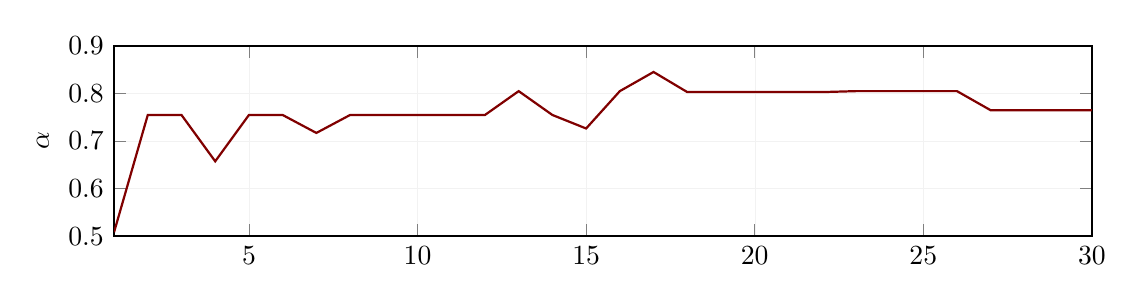
\begin{tikzpicture}
	\begin{axis}[
	%	xlabel={Generation},
	ylabel={$\alpha$},
	xmin=1, xmax=30,
	ymin=0.5, ymax=0.9,
	grid=both,
	grid style={line width=.1pt, draw=gray!10},
	width=14cm,height=4cm,
	xtick={0,5,10,15,20,25,30},
	ytick={0.5,0.6,0.7,0.8,0.9},
	thick]
	
	\addplot[color=Maroon]
	coordinates {
		(1,0.508448976427112)(2,0.754708795645205)(3,0.754708795645205)
		(4,0.657392330450923)(5,0.754708795645205)(6,0.754708795645205)
		(7,0.716973355862945)(8,0.754708795645205)(9,0.754708795645205)
		(10,0.754708795645205)(11,0.754708795645205)(12,0.754708795645205)
		(13,0.804793959442481)(14,0.754708795645205)(15,0.726326548396839)
		(16,0.804793959442481)(17,0.845033657414605)(18,0.802781974543875)
		(19,0.802781974543875)(20,0.802781974543875)(21,0.802781974543875)
		(22,0.802781974543875)(23,0.804793959442481)(24,0.804793959442481)
		(25,0.804793959442481)(26,0.804793959442481)(27,0.764554261470357)
		(28,0.764554261470357)(29,0.764554261470357)(30,0.764554261470357)
	};
	\end{axis}
	\end{tikzpicture}
	
	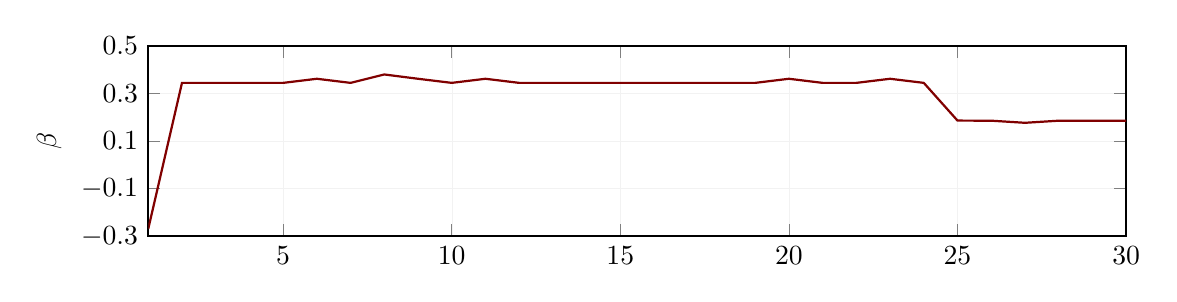
\begin{tikzpicture}
	\begin{axis}[
	%	xlabel={Generation},
	ylabel={$\beta$},
	xmin=1, xmax=30,
	ymin=-0.3, ymax=0.5,
	grid=both,
	grid style={line width=.1pt, draw=gray!10},
	width=14cm,height=4cm,
	xtick={0,5,10,15,20,25,30},
	ytick={-0.3,-0.1,0.1,0.3,0.5},
	thick]
	
	\addplot[color=Maroon]
	coordinates {
		(1,-0.268822537450358)(2,0.344310428956600)(3,0.344310428956600)
		(4,0.344310428956600)(5,0.344310428956600)(6,0.361525950404430)
		(7,0.344310428956600)(8,0.379602247924651)(9,0.361525950404430)
		(10,0.344310428956600)(11,0.361525950404430)(12,0.344310428956600)
		(13,0.344310428956600)(14,0.344310428956600)(15,0.344310428956600)
		(16,0.344310428956600)(17,0.344310428956600)(18,0.344310428956600)
		(19,0.344310428956600)(20,0.361525950404430)(21,0.344310428956600)
		(22,0.344310428956600)(23,0.361525950404430)(24,0.344310428956600)
		(25,0.185855452192517)(26,0.185390813562035)(27,0.176562679582891)
		(28,0.185390813562035)(29,0.185390813562035)(30,0.185390813562035)
	};
	\end{axis}
	\end{tikzpicture}
	
	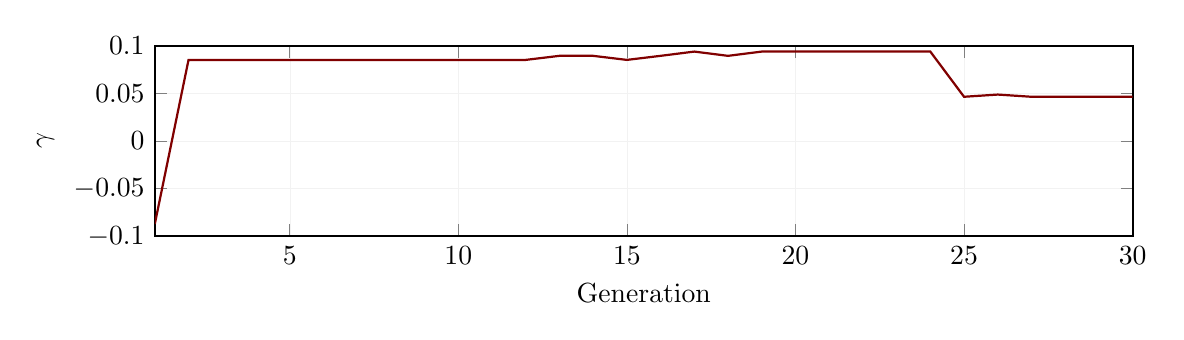
\begin{tikzpicture}
	\begin{axis}[
	xlabel={Generation},
	ylabel={$\gamma$},
	yticklabel style={/pgf/number format/fixed},
	xmin=1, xmax=30,
	ymin=-0.1, ymax=0.1,
	grid=both,
	grid style={line width=.1pt, draw=gray!10},
	width=14cm,height=4cm,
	xtick={0,5,10,15,20,25,30},
	ytick={-0.1,-0.05,0,0.05,0.1},
	thick]
	
	\addplot[color=Maroon]
	coordinates {
		(1,-0.0871709478837318)(2,0.0852051419429015)(3,0.0852051419429015)
		(4,0.0852051419429015)(5,0.0852051419429015)(6,0.0852051419429015)
		(7,0.0852051419429015)(8,0.0852051419429015)(9,0.0852051419429015)
		(10,0.0852051419429015)(11,0.0852051419429015)(12,0.0852051419429015)
		(13,0.0894653990400466)(14,0.0894653990400466)(15,0.0852051419429015)
		(16,0.0894653990400466)(17,0.0939386689920489)(18,0.0894653990400466)
		(19,0.0939386689920489)(20,0.0939386689920489)(21,0.0939386689920489)
		(22,0.0939386689920489)(23,0.0939386689920489)(24,0.0939386689920489)
		(25,0.0464759550397010)(26,0.0487997527916861)(27,0.0464759550397010)
		(28,0.0464759550397010)(29,0.0464759550397010)(30,0.0464759550397010)
	};
	\end{axis}
	\end{tikzpicture}
	
	\caption{Genetic Algorithm -- Classic Bouc-Wen Model \newline (Random crossover)}
	\label{fig:ga_classic_rand}
\end{figure}


\begin{table}[H]
	\centering
	\begin{tabular}{l c c c c}
		\toprule
		\textbf{Parameter}		& $A$	& $\alpha$	& $\beta$	& $\gamma$ 	\\ \midrule
		\textbf{Final value}	& $0.76158$	& $0.76455$	& $0.18539$ & $0.04647$	\\ \bottomrule
	\end{tabular}
	\caption{Random crossover -- Final values (Classic Bouc-Wen model)}
	\label{tab:ga_classic_random_final}
\end{table}

A series of sharp changes is noticeable in Figure~\ref{fig:ga_classic_rand}.
As said beforehand, this behaviour is due to the fact that the set of chromosomes
obtainable by the individual in the population is fixed to the initial one.

Nonetheless it is possible to notice that the variables $\beta$ and $\gamma$
are the first to settle to fairly consistent values, up until generation 25.
This behaviour is probably due to the current best individual being near a local optimum.

The final values for each parameter using this crossover strategy
are in Table~\ref{tab:ga_classic_random_final}.

\begin{figure}[H]
	\centering
	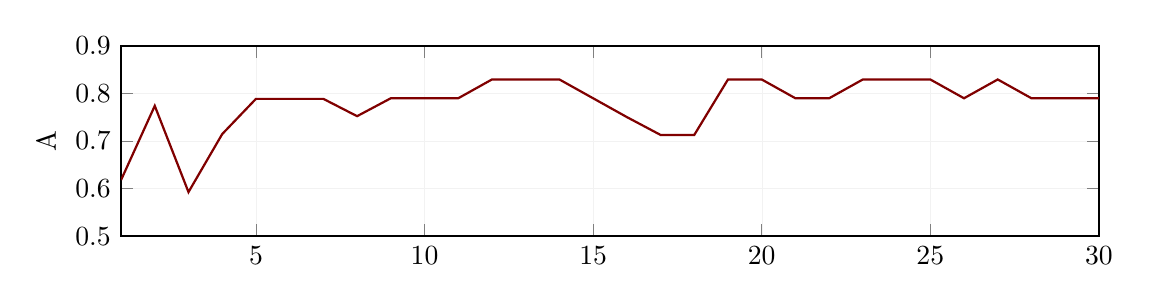
\begin{tikzpicture}
	\begin{axis}[
	%	xlabel={Generation},
	ylabel={A},
	xmin=1, xmax=30,
	ymin=0.5, ymax=0.9,
	grid=both,
	grid style={line width=.1pt, draw=gray!10},
	width=14cm,height=4cm,
	xtick={0,5,10,15,20,25,30},
	ytick={0.5,0.6,0.7,0.8,0.9},
	thick]
	
	\addplot[color=Maroon]
	coordinates {
		(1,0.618086069866413)(2,0.773856623996490)(3,0.592746940707517)
		(4,0.714602293601890)(5,0.788559995124738)(6,0.788559995124738)
		(7,0.788559995124738)(8,0.752212940633569)(9,0.789823587665247)
		(10,0.789823587665247)(11,0.789823587665247)(12,0.829314767048510)
		(13,0.829314767048510)(14,0.829314767048510)(15,0.789823587665247)
		(16,0.750332408281985)(17,0.712815787867886)(18,0.712815787867886)
		(19,0.829314767048510)(20,0.829314767048510)(21,0.789823587665247)
		(22,0.789823587665247)(23,0.829314767048510)(24,0.829314767048510)
		(25,0.829314767048510)(26,0.789823587665247)(27,0.829314767048510)
		(28,0.789823587665247)(29,0.789823587665247)(30,0.789823587665247)
	};
	\end{axis}
	\end{tikzpicture}
	
	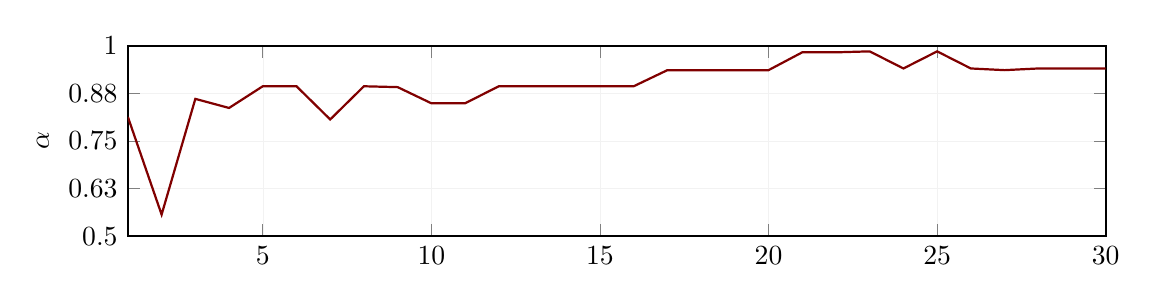
\begin{tikzpicture}
	\begin{axis}[
	%	xlabel={Generation},
	ylabel={$\alpha$},
	xmin=1, xmax=30,
	ymin=0.5, ymax=1,
	grid=both,
	grid style={line width=.1pt, draw=gray!10},
	width=14cm,height=4cm,
	xtick={0,5,10,15,20,25,30},
	ytick={0.5,0.625,0.75,0.875,1},
	thick]
	
	\addplot[color=Maroon]
	coordinates {
		(1,0.813187272905702)(2,0.556820971784476)(3,0.860684845546224)
		(4,0.836803572892517)(5,0.893766789568932)(6,0.893766789568932)
		(7,0.806624527585961)(8,0.893766789568932)(9,0.891532372595010)
		(10,0.849078450090485)(11,0.849078450090485)(12,0.893766789568932)
		(13,0.893766789568932)(14,0.893766789568932)(15,0.893766789568932)
		(16,0.893766789568932)(17,0.936108991224760)(18,0.936108991224760)
		(19,0.936108991224760)(20,0.936108991224760)(21,0.982914440785998)
		(22,0.982914440785998)(23,0.985377885499748)(24,0.940500000000000)
		(25,0.985377885499748)(26,0.940500000000000)(27,0.936108991224760)
		(28,0.940500000000000)(29,0.940500000000000)(30,0.940500000000000)
	};
	\end{axis}
	\end{tikzpicture}
	
	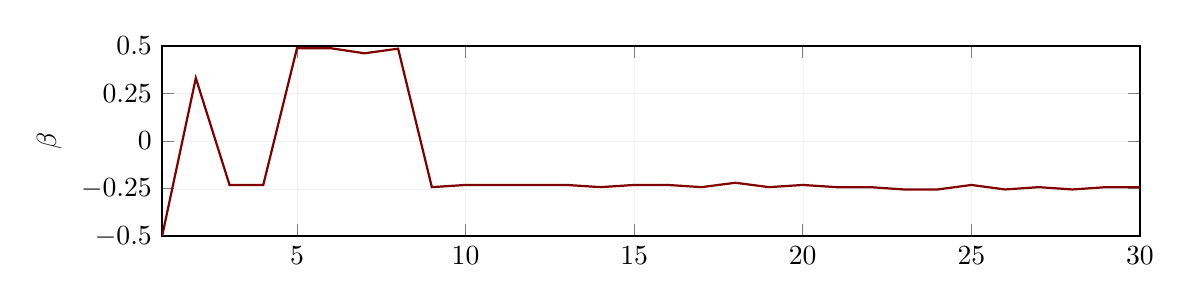
\begin{tikzpicture}
	\begin{axis}[
	%	xlabel={Generation},
	ylabel={$\beta$},
	xmin=1, xmax=30,
	ymin=-0.5, ymax=0.5,
	grid=both,
	grid style={line width=.1pt, draw=gray!10},
	width=14cm,height=4cm,
	xtick={0,5,10,15,20,25,30},
	ytick={-0.5,-0.25,0,0.25,0.5},
	thick]
	
	\addplot[color=Maroon]
	coordinates {
		(1,-0.499357514523178)(2,0.330664545640134)(3,-0.230611577461169)
		(4,-0.230611577461169)(5,0.487411160746289)(6,0.487411160746289)
		(7,0.460700703070708)(8,0.484948108495482)(9,-0.242142156334227)
		(10,-0.230611577461169)(11,-0.230611577461169)(12,-0.230611577461169)
		(13,-0.230611577461169)(14,-0.242142156334227)(15,-0.230611577461169)
		(16,-0.230611577461169)(17,-0.242142156334227)(18,-0.219080998588110)
		(19,-0.242142156334227)(20,-0.230611577461169)(21,-0.242142156334227)
		(22,-0.242142156334227)(23,-0.254249264150938)(24,-0.254249264150938)
		(25,-0.230611577461169)(26,-0.254249264150938)(27,-0.242142156334227)
		(28,-0.254249264150938)(29,-0.242142156334227)(30,-0.242142156334227)
	};
	\end{axis}
	\end{tikzpicture}
	
	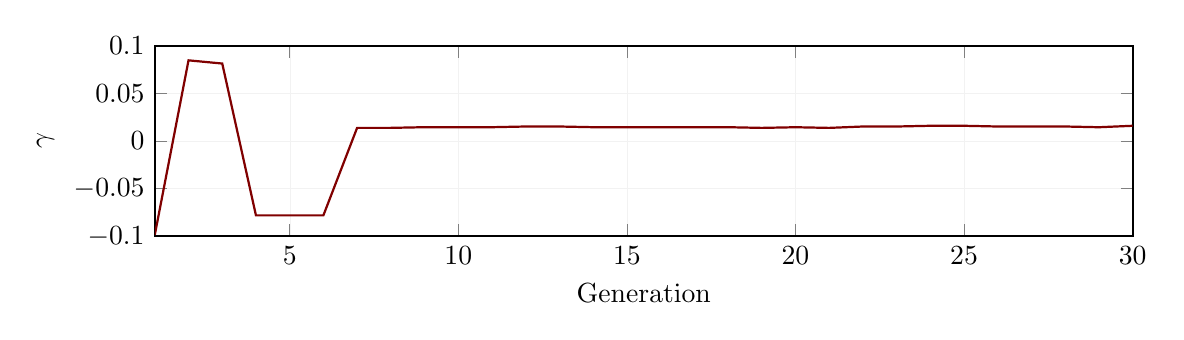
\begin{tikzpicture}
	\begin{axis}[
	xlabel={Generation},
	ylabel={$\gamma$},
	yticklabel style={/pgf/number format/fixed},
	xmin=1, xmax=30,
	ymin=-0.1, ymax=0.1,
	grid=both,
	grid style={line width=.1pt, draw=gray!10},
	width=14cm,height=4cm,
	xtick={0,5,10,15,20,25,30},
	ytick={-0.1,-0.05,0,0.05,0.1},
	thick]
	
	\addplot[color=Maroon]
	coordinates {
		(1,-0.0985378305342493)(2,0.0847351667259024)(3,0.0813828498620047)
		(4,-0.0780844050799008)(5,-0.0780844050799008)(6,-0.0780844050799008)
		(7,0.0138301733936949)(8,0.0138301733936949)(9,0.0145216820633796)
		(10,0.0145216820633796)(11,0.0145216820633796)(12,0.0152477661665486)
		(13,0.0152477661665486)(14,0.0145216820633796)(15,0.0145216820633796)
		(16,0.0145216820633796)(17,0.0145216820633796)(18,0.0145216820633796)
		(19,0.0137955979602107)(20,0.0144853778582212)(21,0.0137955979602107)
		(22,0.0152477661665486)(23,0.0152477661665486)(24,0.0160101544748761)
		(25,0.0160101544748761)(26,0.0152477661665486)(27,0.0152477661665486)
		(28,0.0152477661665486)(29,0.0144853778582212)(30,0.0160101544748761)
	};
	\end{axis}
	\end{tikzpicture}
	
	\caption{Genetic Algorithm -- Classic Bouc-Wen Model \newline (Weighted~crossover)}
	\label{fig:ga_classic_w}
\end{figure}

As for the random crossover strategy, the weighted crossover strategy
operates on the closed set of initial chromosome values, but combines
them judging the fit value of the individuals instead of doing it randomly.

The most important difference between these two results is the fact that
it takes fewer generations to reach what may be a global optimum.
This is especially noticeable in Figure~\ref{fig:ga_classic_w},
as the parameters $\beta$ and $\gamma$ stabilize on similar values
around generation 10 and 7, respectively.

The final values for each parameter using this crossover strategy
are in Table~\ref{tab:ga_classic_weighted_final}.

\begin{table}[H]
	\centering
	\begin{tabular}{l c c c c}
		\toprule
		\textbf{Parameter}		& $A$	& $\alpha$	& $\beta$	& $\gamma$ 	\\ \midrule
		\textbf{Final value}	& $0.78982$	& $0.94050$	& $-0.24214$ & $0.01601$	\\ \bottomrule
	\end{tabular}
	\caption{Weighted crossover -- Final values (Classic Bouc-Wen model)}
	\label{tab:ga_classic_weighted_final}
\end{table}

\begin{figure}[H]
	\centering
	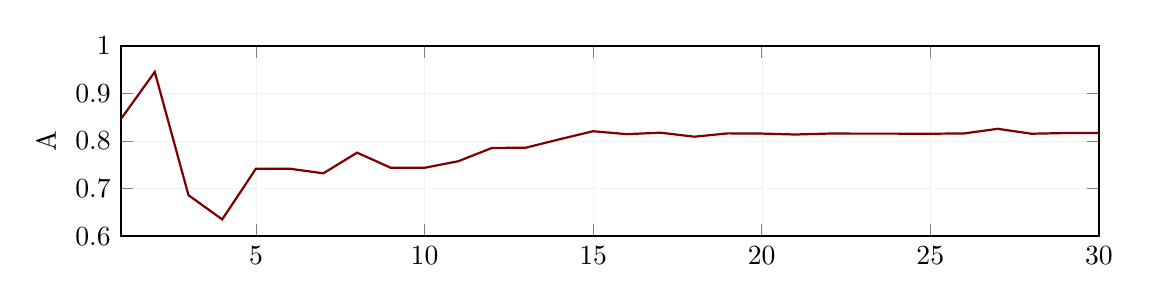
\begin{tikzpicture}
	\begin{axis}[
%	xlabel={Generation},
	ylabel={A},
	xmin=1, xmax=30,
	ymin=0.6, ymax=1,
    grid=both,
	grid style={line width=.1pt, draw=gray!10},
	width=14cm,height=4cm,
	xtick={0,5,10,15,20,25,30},
	ytick={0.6,0.7,0.8,0.9,1},
	thick
	]
	
	\addplot[
	color=Maroon
	]
	coordinates {
		(1,0.846617612122516)(2,0.945169707132505)(3,0.686185321911442)
		(4,0.635391880114644)(5,0.741875275061889)(6,0.741875275061889)
		(7,0.732155512378616)(8,0.775578685813760)(9,0.743785928735175)
		(10,0.743785928735175)(11,0.757533941052583)(12,0.785476285913808)
		(13,0.785895602859595)(14,0.803612148048867)(15,0.820560794469268)
		(16,0.814418644574798)(17,0.817525500030851)(18,0.809111673028719)
		(19,0.816070097329638)(20,0.815637998888346)(21,0.813705102461688)
		(22,0.815690431932833)(23,0.815517137553180)(24,0.815517137553180)
		(25,0.815353069534198)(26,0.815868881606655)(27,0.825692496498711)
		(28,0.815308753557013)(29,0.816773883289793)(30,0.816995005947158)
	};
	
	\end{axis}
	\end{tikzpicture}

	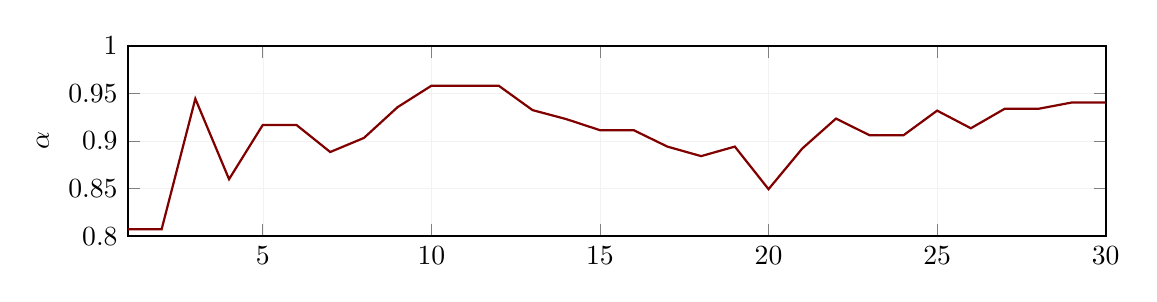
\begin{tikzpicture}
	\begin{axis}[
	ylabel={$\alpha$},
	xmin=1, xmax=30,
	ymin=0.8, ymax=1,
	grid=both,
	grid style={line width=.1pt, draw=gray!10},
	width=14cm,height=4cm,
	xtick={0,5,10,15,20,25,30},
	ytick={0.8,0.85,0.9,0.95,1},
	thick
	]
	
	\addplot[
	color=Maroon
	]
	coordinates {
		(1,0.807304104758228)(2,0.807304104758228)(3,0.944409289353833)
		(4,0.859921322048516)(5,0.916860139599848)(6,0.916860139599848)
		(7,0.888463783458492)(8,0.903226651793137)(9,0.935606267534623)
		(10,0.958038312299642)(11,0.958038312299642)(12,0.958038312299642)
		(13,0.932466246978050)(14,0.923030423935558)(15,0.911376532519616)
		(16,0.911376532519616)(17,0.894144784683887)(18,0.884143786894717)
		(19,0.894144784683887)(20,0.849437545449693)(21,0.892107817478434)
		(22,0.923568595351979)(23,0.906003036557694)(24,0.906003036557694)
		(25,0.931929326970839)(26,0.913402075446632)(27,0.933810236925943)		(28,0.933810236925943)(29,0.940500000000000)(30,0.940500000000000)	
	};
	
	\end{axis}
	\end{tikzpicture}

	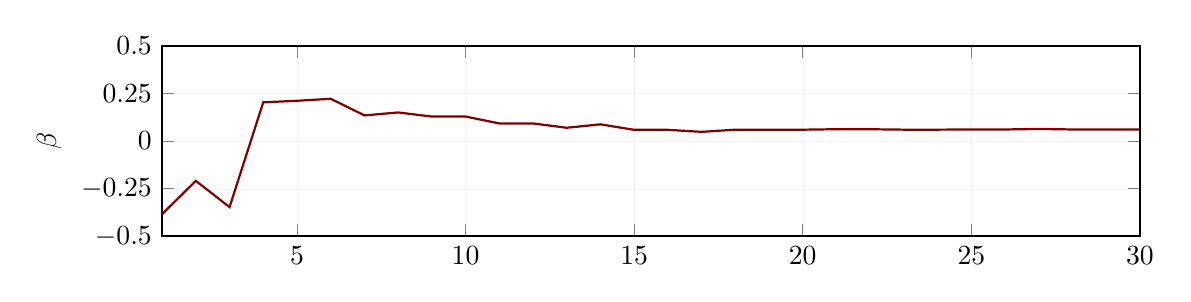
\begin{tikzpicture}
	\begin{axis}[
	ylabel={$\beta$},
	xmin=1, xmax=30,
	ymin=-0.5, ymax=0.5,
	grid=both,
	grid style={line width=.1pt, draw=gray!10},
	width=14cm,height=4cm,
	xtick={0,5,10,15,20,25,30},
	ytick={-0.5,-0.25,0,0.25,0.5},
	thick
	]
	
	\addplot[
	color=Maroon
	]
	coordinates {
	(1,-0.383570164339162)(2,-0.209067239339800)(3,-0.346945447394620)
	(4,0.203314842137601)(5,0.211317604599334)(6,0.221883484829301)
	(7,0.134575000183786)(8,0.150040172965104)(9,0.128552630840732)
	(10,0.128552630840732)(11,0.0924247538988270)(12,0.0924247538988270)
	(13,0.0696849041430703)(14,0.0876972336644854)(15,0.0588128772541681)
	(16,0.0588128772541681)(17,0.0481057225684876)(18,0.0596059416498790)
	(19,0.0596059416498790)(20,0.0595554726646533)(21,0.0620742434800105)
	(22,0.0619325894560293)(23,0.0597591278277150)(24,0.0597591278277150)
	(25,0.0606863986765927)(26,0.0607556620243750)(27,0.0633912791535188)
	(28,0.0607681427718138)(29,0.0609861619403020)(30,0.0607868744138922)
	};
	\end{axis}
	\end{tikzpicture}

	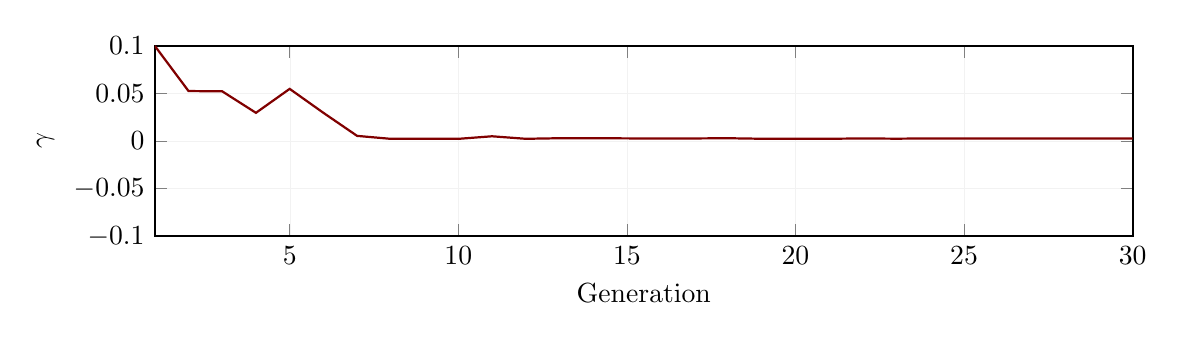
\begin{tikzpicture}
	\begin{axis}[
	yticklabel style={/pgf/number format/fixed},
	xlabel={Generation},
	ylabel={$\gamma$},
	xmin=1, xmax=30,
	ymin=-0.1, ymax=0.1,
	grid=both,	      
	scaled y ticks = false,		
	grid style={line width=.1pt, draw=gray!10},
	width=14cm,height=4cm,
	xtick={0,5,10,15,20,25,30},
	ytick={-0.1,-0.05,0,0.05,0.1},
	thick
	]
	
	\addplot[
	color=Maroon
	]
	coordinates {
		(1,0.0999415052821818)(2,0.0524929987796510)(3,0.0521746568499797)
		(4,0.0296226513494849)(5,0.0547827566575863)(6,0.0296226513494849)
		(7,0.00540555464037581)(8,0.00228429919009436)(9,0.00228429919009436)
		(10,0.00228429919009436)(11,0.00498059078371382)(12,0.00234127234304952)
		(13,0.00294145297861557)(14,0.00294145297861557)(15,0.00277665812010004)
		(16,0.00261202366681348)(17,0.00271992213742177)(18,0.00293279836879291)
		(19,0.00237952420577038)(20,0.00237952420577038)(21,0.00237952420577038)
		(22,0.00269933620416253)(23,0.00245930491141351)(24,0.00273011191599481)
		(25,0.00273011191599481)(26,0.00257043305522086)(27,0.00262062997493030)
		(28,0.00261361171864668)(29,0.00261407624380850)(30,0.00273011191599481)
	};
	\end{axis}
	\end{tikzpicture}
	\caption{Genetic Algorithm -- Classic Bouc-Wen Model (Proportional crossover)}
	\label{fig:ga_classic_prop}
\end{figure}

In contrast to the parameter trends of random and weighted crossover strategies,
the proportional crossover strategy shows a smoother trend. 
This is especially noticeable for parameters $A$, $\beta$ and $\gamma$.

As for the weighted crossover method, it is possible to see an almost
immediate setting of parameters $\beta$ and $\gamma$, as it happens
for both around generation 7.

The final values for each parameter using this crossover strategy
are in Table~\ref{tab:ga_classic_prop_final}.

\begin{table}[H]
	\centering
	\begin{tabular}{l c c c c}
		\toprule
		\textbf{Parameter}		& $A$	& $\alpha$	& $\beta$	& $\gamma$ 	\\ \midrule
		\textbf{Final value}	& $0.81699$	& $0.94050$	& $0.06078$ & $0.00273$	\\ \bottomrule
	\end{tabular}
	\caption{Weighted crossover -- Final values (Classic Bouc-Wen model)}
	\label{tab:ga_classic_prop_final}
\end{table}

Figure~\ref{fig:ga_classic_res} shows how the hysteresis loop behaves
with the final parameters present in Table~\ref{tab:ga_classic_prop_final}.

\begin{figure}[H]
	\centering
	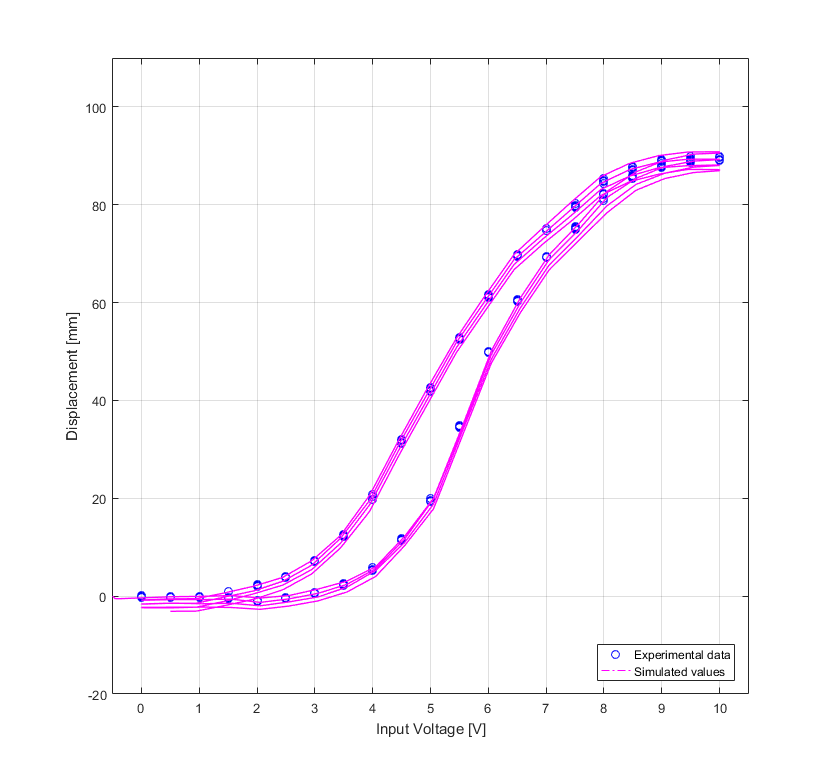
\includegraphics[width=\linewidth]{Images/ga_prop_final}
	\caption{Hysteresis loop result -- Genetic Algorithm's parameters (classic Bouc-Wen model, proportional crossover approach)}
	\label{fig:ga_classic_res}
\end{figure}

\subsubsection{Modified Firefly Algorithm -- Classic Bouc-Wen Model}

Table~\ref{tab:mfa_classic_params} contains the parameters used for the
Modified Firefly Algorithm approach. 

\begin{table}[H]
	\centering
	\begin{tabular}{c c}
		\toprule
		\textbf{Parameter} & \textbf{Value} \\ \toprule
		$N$			& $30$ \\
		$G$			& $30$ \\
		$d$			& $4$  \\
		$L$			& $\left[0, 0.5, -0.5, -0.5\right]$ \\
		$U$			& $\left[2, 0.99, 0.5, 0.5\right]$ \\ 
		$a$			& $1.1$ \\
		$b$			& $0.3$ \\ \bottomrule
	\end{tabular}
	\caption{Parameters for the Modified Firefly Algorithm approach -- Classic Bouc-Wen model}
	\label{tab:mfa_classic_params}
\end{table}

Figure~\ref{fig:mfa_classic_trend} shows the trend of Bouc-Wen parameters
$A$, $\alpha$, $\beta$ and $\gamma$ using the Modified Firefly Algorithm.

\begin{figure}[H]
	\centering
	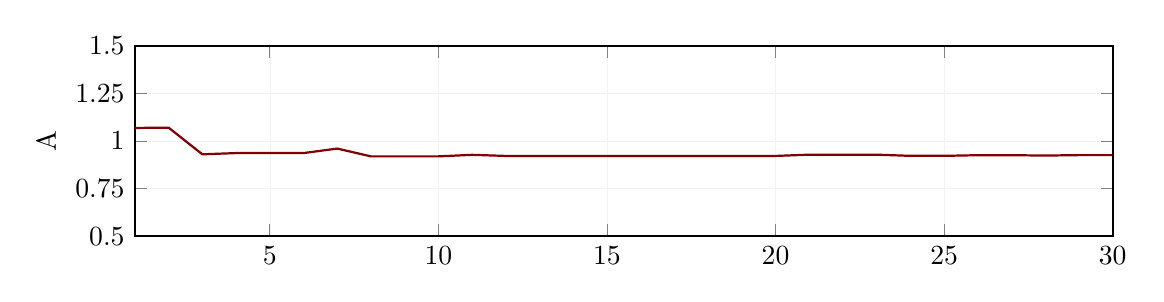
\begin{tikzpicture}
	\begin{axis}[
	ylabel={A},
	xmin=1, xmax=30,
	ymin=0.5, ymax=1.5,
	grid=both,
	grid style={line width=.1pt, draw=gray!10},
	width=14cm,height=4cm,
	xtick={0,5,10,15,20,25,30},
	ytick={0.5,0.75,1,1.25,1.5},
	thick]
	
	\addplot[color=Maroon]
	coordinates {
		(1,1.06869060925092)(2,1.07031310017167)(3,0.930245427082584)
		(4,0.936679613305865)(5,0.936679613305865)(6,0.936679613305865)
		(7,0.960367546450692)(8,0.919402031004002)(9,0.919402031004002)
		(10,0.919402031004002)(11,0.927525757993710)(12,0.921703837572361)
		(13,0.921703837572361)(14,0.921703837572361)(15,0.921703837572361)
		(16,0.921703837572361)(17,0.921703837572361)(18,0.921703837572361)
		(19,0.921703837572361)(20,0.921703837572361)(21,0.928354088631171)
		(22,0.928354088631171)(23,0.928354088631171)(24,0.922151802845455)
		(25,0.922151802845455)(26,0.925594763845607)(27,0.925594763845607)
		(28,0.923707972405618)(29,0.925963112330994)(30,0.925963112330994)
	};
	
	\end{axis}
	\end{tikzpicture}
	
	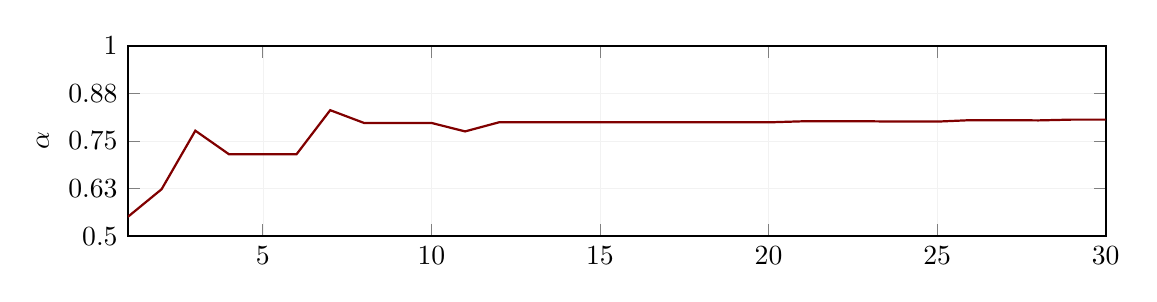
\begin{tikzpicture}
	\begin{axis}[
	ylabel={$\alpha$},
	xmin=1, xmax=30,
	ymin=0.5, ymax=1,
	grid=both,
	grid style={line width=.1pt, draw=gray!10},
	width=14cm,height=4cm,
	xtick={0,5,10,15,20,25,30},
	ytick={0.5,0.625,0.75,0.875,1},
	thick
	]
	
	\addplot[
	color=Maroon
	]
	coordinates {
		(1,0.550976413814157)(2,0.623490876234948)(3,0.777128984609912)
		(4,0.715106724722959)(5,0.715106724722959)(6,0.715106724722959)
		(7,0.830987001080587)(8,0.797556605573597)(9,0.797556605573597)
		(10,0.797556605573597)(11,0.775232834887466)(12,0.799023435255703)
		(13,0.799023435255703)(14,0.799023435255703)(15,0.799023435255703)
		(16,0.799023435255703)(17,0.799023435255703)(18,0.799023435255703)
		(19,0.799023435255703)(20,0.799023435255703)(21,0.801751730639454)
		(22,0.801751730639454)(23,0.801751730639454)(24,0.800992660349603)
		(25,0.800992660349603)(26,0.804812870702901)(27,0.804812870702901)
		(28,0.804148278131032)(29,0.806209042629755)(30,0.806209042629755)	
	};
	
	\end{axis}
	\end{tikzpicture}
	
	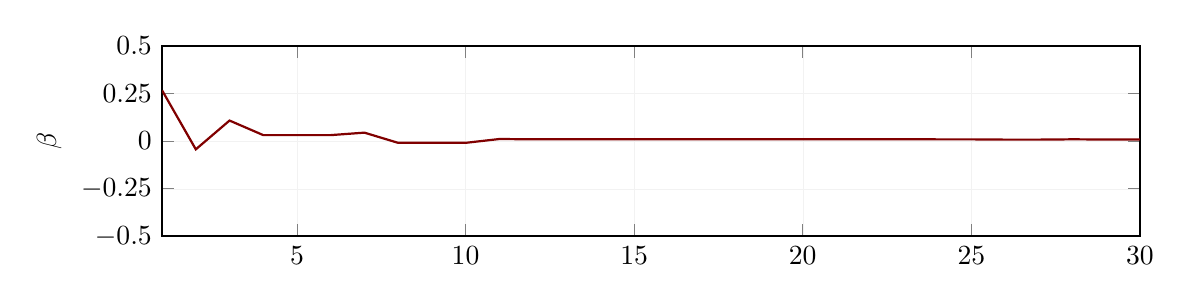
\begin{tikzpicture}
	\begin{axis}[
	ylabel={$\beta$},
	xmin=1, xmax=30,
	ymin=-0.5, ymax=0.5,
	grid=both,
	grid style={line width=.1pt, draw=gray!10},
	width=14cm,height=4cm,
	xtick={0,5,10,15,20,25,30},
	ytick={-0.5,-0.25,0,0.25,0.5},
	thick
	]
	
	\addplot[color=Maroon]
	coordinates {
		(1,0.266001570301431)(2,-0.0435908362222465)(3,0.107569352046298)
		(4,0.0310859001662921)(5,0.0310859001662921)(6,0.0310859001662921)
		(7,0.0440423469108267)(8,-0.00952233930470358)(9,-0.00952233930470358)
		(10,-0.00952233930470358)(11,0.0105856910126518)(12,0.00911806671740018)
		(13,0.00911806671740018)(14,0.00911806671740018)(15,0.00911806671740018)
		(16,0.00911806671740018)(17,0.00911806671740018)(18,0.00911806671740018)
		(19,0.00911806671740018)(20,0.00911806671740018)(21,0.00915095605160595)
		(22,0.00915095605160595)(23,0.00915095605160595)(24,0.00878879253828613)
		(25,0.00878879253828613)(26,0.00740178743614416)(27,0.00740178743614416)
		(28,0.00901025687938335)(29,0.00806867272972272)(30,0.00806867272972272)
	};
	\end{axis}
	\end{tikzpicture}
	
	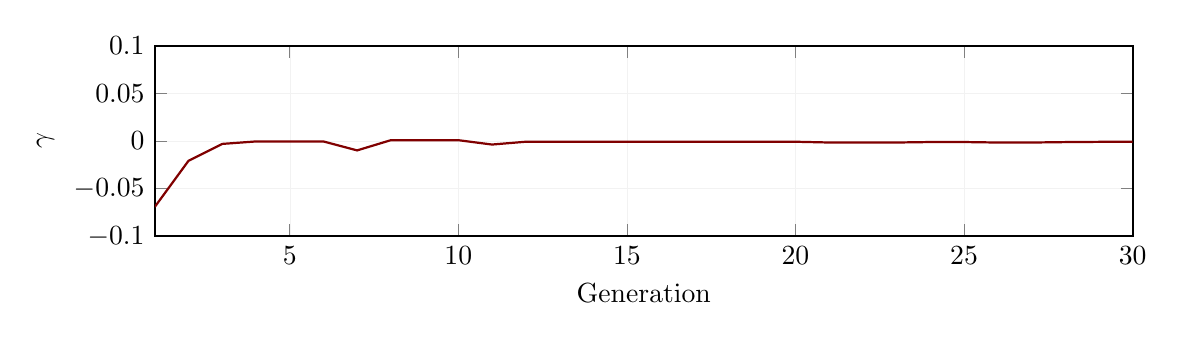
\begin{tikzpicture}
	\begin{axis}[
	yticklabel style={/pgf/number format/fixed},
	xlabel={Generation},
	ylabel={$\gamma$},
	xmin=1, xmax=30,
	ymin=-0.1, ymax=0.1,
	grid=both,	      
	scaled y ticks = false,		
	grid style={line width=.1pt, draw=gray!10},
	width=14cm,height=4cm,
	xtick={0,5,10,15,20,25,30},
	ytick={-0.1,-0.05,0,0.05,0.1},
	thick
	]
	
	\addplot[color=Maroon]
	coordinates {
		(1,-0.0691733544526680)(2,-0.0207321319806590)(3,-0.00302967769376153)
		(4,-0.000441510968489555)(5,-0.000441510968489555)(6,-0.000441510968489555)
		(7,-0.00983967294117288)(8,0.000890856083589599)(9,0.000890856083589599)
		(10,0.000890856083589599)(11,-0.00369252054175541)(12,-0.000756154478913090)
		(13,-0.000756154478913090)(14,-0.000756154478913090)(15,-0.000756154478913090)
		(16,-0.000756154478913090)(17,-0.000756154478913090)(18,-0.000756154478913090)
		(19,-0.000756154478913090)(20,-0.000756154478913090)(21,-0.00155480896080897)
		(22,-0.00155480896080897)(23,-0.00155480896080897)(24,-0.00106283248509903)
		(25,-0.00106283248509903)(26,-0.00157157076493920)(27,-0.00157157076493920)
		(28,-0.00112928693805224)(29,-0.000866865925248103)(30,-0.000866865925248103)
	};
	\end{axis}
	\end{tikzpicture}
	\caption{Modified Firefly Algorithm -- Classic Bouc-Wen Model}
	\label{fig:mfa_classic_trend}
\end{figure}

Conversely to the Genetic Algorithm, the Modified Firefly Approach
has reached good fit values in each run of the algorithm for the classic Bouc-Wen model.

Moreover, it immediately stands out how the trend of the four parameters
is smoother with respect to the GA approach, for each of the three crossover strategies.

The final values found for each parameter using the MFA approach are shown
in Table~\ref{tab:mfa_final_classic}.

\begin{table}[H]
	\centering
	\begin{tabular}{l c c c c}
		\toprule
		\textbf{Parameter}		& $A$	& $\alpha$	& $\beta$	& $\gamma$ 	\\ \midrule
		\textbf{Final value}	& $0.92596$	& $0.80620$	& $0.00806$ & $-0.00086$ \\
		\bottomrule
	\end{tabular}
	\caption{Modified Firefly Algorithm -- Final values (Classic Bouc-Wen model)}
	\label{tab:mfa_final_classic}
\end{table}

Figure~\ref{fig:mfa_classic_hys} shows how the hysteresis loop behaves
with the final parameters of Table~\ref{tab:mfa_final_classic}.

\begin{figure}[H]
	\centering
	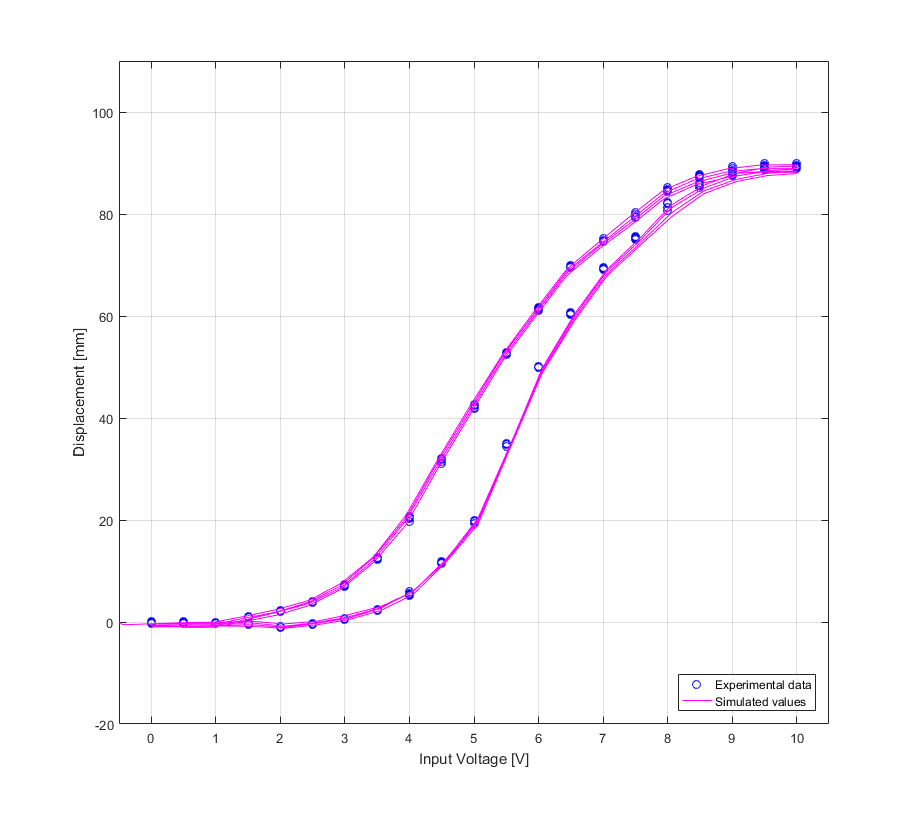
\includegraphics[width=\linewidth]{Images/mfa_prop_final}
	\caption{Hysteresis loop result using Modified Firefly Algorithm parameters (classic Bouc-Wen model)}
	\label{fig:mfa_classic_hys}
\end{figure}

\subsubsection{Particle Swarm Optimization -- Classic Bouc-Wen Model}

Table~\ref{tab:pso_classic_params} contains the parameters used for the
Particle Swarm Optimization approach. 

\begin{table}[H]
	\centering
	\begin{tabular}{c c}
		\toprule
		\textbf{Parameter} & \textbf{Value} \\ \toprule
		$N$			& $10$ \\
		$G$			& $30$ \\
		$d$			& $4$  \\
		$L$			& $\left[0, 0, -0.5, -0.5\right]$ \\
		$U$			& $\left[2, 0.9, 0.5, 0.5\right]$ \\ 
		$a$			& $1.1$ \\
		$b$			& $0.3$ \\ 
		$c_1$		& $2$	\\
		$c_2$		& $2$	\\ 
		$V_{max}$	& $\left[20,20,20,20\right]$ \\ \bottomrule
	\end{tabular}
	\caption{Parameters for the Particle Swarm Optimization approach -- Classic Bouc-Wen model}
	\label{tab:pso_classic_params}
\end{table}

\begin{figure}[H]
	\centering
	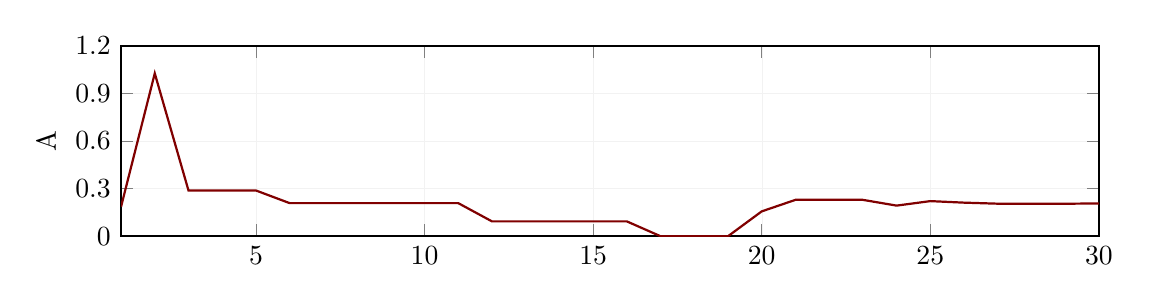
\begin{tikzpicture}
	\begin{axis}[
	ylabel={A},
	xmin=1, xmax=30,
	ymin=0, ymax=1.2,
	grid=both,
	grid style={line width=.1pt, draw=gray!10},
	width=14cm,height=4cm,
	xtick={0,5,10,15,20,25,30},
	ytick={0,0.3,0.6,0.9,1.2},
	thick]
	
	\addplot[color=Maroon]
	coordinates {
		(1,0.185863237644164)(2,1.02632063487202)(3,0.288380617321494)
		(4,0.288380617321494)(5,0.288380617321494)(6,0.208683447421379)
		(7,0.208683447421379)(8,0.208683447421379)(9,0.208683447421379)
		(10,0.208683447421379)(11,0.208683447421379)(12,0.0936642393040911)
		(13,0.0936642393040911)(14,0.0936642393040911)(15,0.0936642393040911)
		(16,0.0936642393040911)(17,0)(18,0)(19,0)(20,0.156627431188312)
		(21,0.229294550577293)(22,0.229294550577293)(23,0.229294550577293)
		(24,0.193037101921784)(25,0.221355518470106)(26,0.211708341239334)
		(27,0.205145183300729)(28,0.205145183300729)(29,0.204949632696870)
		(30,0.206511896266668)
	};
	
	\end{axis}
	\end{tikzpicture}
	
	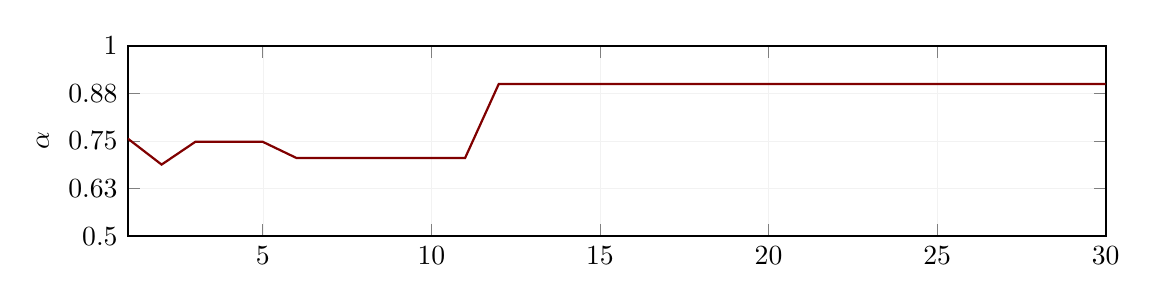
\begin{tikzpicture}
	\begin{axis}[
	ylabel={$\alpha$},
	xmin=1, xmax=30,
	ymin=0.5, ymax=1,
	grid=both,
	grid style={line width=.1pt, draw=gray!10},
	width=14cm,height=4cm,
	xtick={0,5,10,15,20,25,30},
	ytick={0.5,0.625,0.75,0.875,1},
	thick
	]
	
	\addplot[
	color=Maroon
	]
	coordinates {
		(1,0.756220545192621)(2,0.688144395916196)(3,0.747916747206713)
		(4,0.747916747206713)(5,0.747916747206713)(6,0.705433678358796)
		(7,0.705433678358796)(8,0.705433678358796)(9,0.705433678358796)
		(10,0.705433678358796)(11,0.705433678358796)(12,0.900000000000000)
		(13,0.900000000000000)(14,0.900000000000000)(15,0.900000000000000)
		(16,0.900000000000000)(17,0.900000000000000)(18,0.900000000000000)
		(19,0.900000000000000)(20,0.900000000000000)(21,0.900000000000000)
		(22,0.900000000000000)(23,0.900000000000000)(24,0.900000000000000)
		(25,0.900000000000000)(26,0.900000000000000)(27,0.900000000000000)
		(28,0.900000000000000)(29,0.900000000000000)(30,0.900000000000000)	
	};
	
	\end{axis}
	\end{tikzpicture}
	
	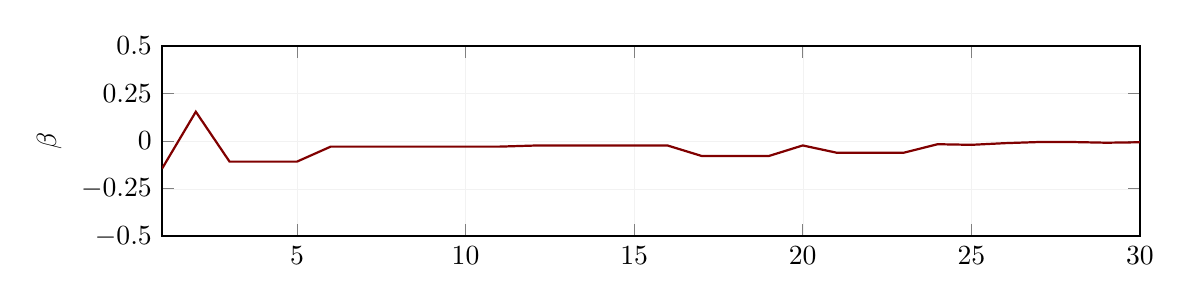
\begin{tikzpicture}
	\begin{axis}[
	ylabel={$\beta$},
	xmin=1, xmax=30,
	ymin=-0.5, ymax=0.5,
	grid=both,
	grid style={line width=.1pt, draw=gray!10},
	width=14cm,height=4cm,
	xtick={0,5,10,15,20,25,30},
	ytick={-0.5,-0.25,0,0.25,0.5},
	thick
	]
	
	\addplot[color=Maroon]
	coordinates {
		(1,-0.144486390209083)(2,0.153809389216694)(3,-0.108100843747831)
		(4,-0.108100843747831)(5,-0.108100843747831)(6,-0.0293705905740140)
		(7,-0.0293705905740140)(8,-0.0293705905740140)(9,-0.0293705905740140)
		(10,-0.0293705905740140)(11,-0.0293705905740140)(12,-0.0239743852941000)
		(13,-0.0239743852941000)(14,-0.0239743852941000)(15,-0.0239743852941000)
		(16,-0.0239743852941000)(17,-0.0782885386391373)(18,-0.0782885386391373)
		(19,-0.0782885386391373)(20,-0.0231738982815848)(21,-0.0611492972263083)
		(22,-0.0611492972263083)(23,-0.0611492972263083)(24,-0.0167300819866512)
		(25,-0.0199168329453418)(26,-0.0111377647330169)(27,-0.00520380574948877)
		(28,-0.00520380574948877)(29,-0.00883235888170176)(30,-0.00650822592915697)
	};
	\end{axis}
	\end{tikzpicture}
	
	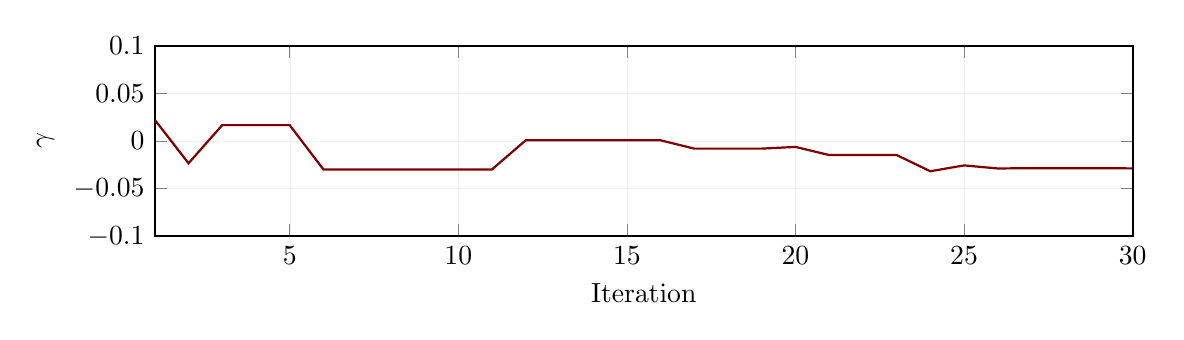
\begin{tikzpicture}
	\begin{axis}[
	yticklabel style={/pgf/number format/fixed},
	xlabel={Iteration},
	ylabel={$\gamma$},
	xmin=1, xmax=30,
	ymin=-0.1, ymax=0.1,
	grid=both,	      
	scaled y ticks = false,		
	grid style={line width=.1pt, draw=gray!10},
	width=14cm,height=4cm,
	xtick={0,5,10,15,20,25,30},
	ytick={-0.1,-0.05,0,0.05,0.1},
	thick
	]
	
	\addplot[color=Maroon]
	coordinates {
		(1,0.0222543785571379)(2,-0.0233438802771272)(3,0.0166923904909300)
		(4,0.0166923904909300)(5,0.0166923904909300)(6,-0.0298037649915088)
		(7,-0.0298037649915088)(8,-0.0298037649915088)(9,-0.0298037649915088)
		(10,-0.0298037649915088)(11,-0.0298037649915088)(12,0.000731539435058728)
		(13,0.000731539435058728)(14,0.000731539435058728)(15,0.000731539435058728)
		(16,0.000731539435058728)(17,-0.00796634020356290)(18,-0.00796634020356290)
		(19,-0.00796634020356290)(20,-0.00618349892532456)(21,-0.0147185482941685)
		(22,-0.0147185482941685)(23,-0.0147185482941685)(24,-0.0317484900349273)
		(25,-0.0256008237924044)(26,-0.0288175678749165)(27,-0.0285119507981094)
		(28,-0.0285119507981094)(29,-0.0285229257459806)(30,-0.0287472123663116)
	};
	\end{axis}
	\end{tikzpicture}
	\caption{Particle Swarm Optimization -- Classic Bouc-Wen Model}
	\label{fig:pso_classic_trend}
\end{figure}

Figure~\ref{fig:pso_classic_trend} shows the trend of Bouc-Wen parameters
using the Particle Swarm Optimization approach~\footnote{The values shown in Figure~\ref{fig:pso_classic_trend}
refer to the particle that attained the best global fit value ($gbest$)
up until that iteration.}.

It is possible to notice that around iteration 15 two of the four parameters,
namely $\alpha$ and $\beta$, have already settled and do not change much for
later iterations. Thus, the particles continue to move in the solution space
mainly on two coordinates. The remaining parameters $A$ and $\gamma$ stabilize
over a certain value around iteration 20 and 25, respectively.

The final values found for each parameter using the PSO approach
are shown in Table~\ref{tab:pso_classic_final}.

\begin{table}[H]
	\centering
	\begin{tabular}{l c c c c}
		\toprule
		\textbf{Parameter}		& $A$	& $\alpha$	& $\beta$	& $\gamma$ 	\\ \midrule
		\textbf{Final value}	& $0.20651$	& $0.9$	& $-0.00650$ & $-0.02874$ \\
		\bottomrule
	\end{tabular}
	\caption{Particle Swarm Optimization -- Final values (Classic Bouc-Wen model)}
	\label{tab:pso_classic_final}
\end{table}

Figure~\ref{fig:pso_classic_hys} displays how the hysteresis loop is shaped
using the final parameters of Table~\ref{tab:pso_classic_final}.

\begin{figure}[H]
	\centering
	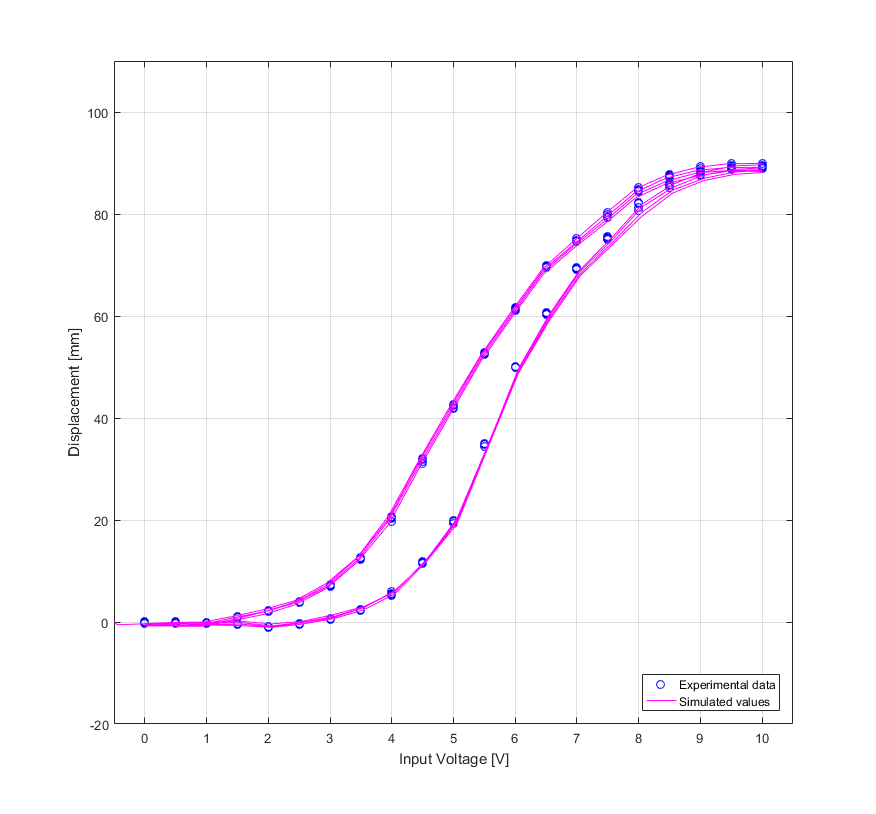
\includegraphics[width=\linewidth]{Images/pso_classic_final}
	\caption{Hysteresis loop result using Particle Swarm Optimization parameters}
	\label{fig:pso_classic_hys}
\end{figure}

\clearpage

\subsection{Solution Comparison -- Generalized Bouc-Wen Model}
\label{sec:5.comp_res_gen}

This Section serves the purpose of comparing the solutions found using the algorithms
described in Sections~\ref{sec:5.ga},~\ref{sec:5.mfa} and~\ref{sec:5.pso}
in order to find suitable parameters for the generalized Bouc-Wen model of hysteresis.

\subsubsection{Genetic Algorithm -- Generalized Bouc-Wen Model}

Table~\ref{tab:ga_gen_params} contains the parameters
used for all three crossover strategies of the Genetic Algorithm approach.

Figures~\ref{fig:ga_gen_rand},~\ref{fig:ga_gen_w} and~\ref{fig:ga_gen_prop}
display the trend of the generalized Bouc-Wen model parameters
$A$, $\alpha$, $\beta_1$, $\beta_2$, $\beta_3$, $\beta_4$, $\beta_5$ and $\beta_6$
depending on the crossover method used~\footnote{
As for the classic model, Figure~\ref{fig:ga_gen_rand} shows, for each generation,
the parameters of the best individual. This will be repeated for subsequent Figures.
}.

The bounds of parameters $\beta_1,\dots,\beta_6$ is narrower than
the bounds used for the classic version of the model. This is due to the fact
that this model is more complex, and thus it is harder to achieve a suitable solution.

It has been observed that the wrong choice of parameters may lead to the
\emph{explosion} of the output, i.e. computational errors add up to a point
where the simulated output diverges. The BIBO stability of the Bouc-Wen
model has been studied and formulated in~\cite{ikhouane2007dynamic}.

\begin{table}[H]
	\centering
	\begin{tabular}{c c}
		\toprule
		\textbf{Parameter} & \textbf{Value} \\ \toprule
		$N$			& $20$ \\
		$G$			& $30$ \\
		$d$			& $8$  \\
		$L$			& $\left[0, 0.5, -0.1, -0.1, -0.1, -0.1, -0.1, -0.1	\right]$ \\
		$U$			& $\left[2, 0.99, 0.5, 0.5, 0.5, 0.5, 0.5, 1			\right]$ \\ 
		$P_{cross}$	& $0.5$ \\
		$P{mut}$	& $0.1$ \\
		$m_m$		& $0.05$ \\	\bottomrule
	\end{tabular}
	\caption{Parameters for the Genetic Algorithm approach -- Generalized Bouc-Wen model}
	\label{tab:ga_gen_params}
\end{table}

% random crossover - generalized bw model
\begin{figure}[H]
	\centering
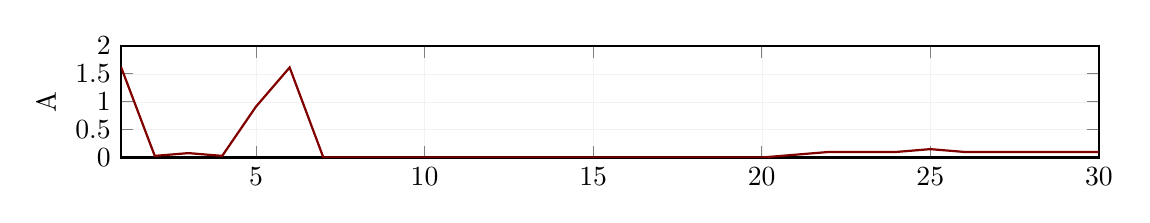
\begin{tikzpicture}
\begin{axis}[
yticklabel style={/pgf/number format/fixed},	
ylabel={A},
xmin=1, xmax=30,
ymin=0, ymax=2,
grid=both,
grid style={line width=.1pt, draw=gray!10},
width=14cm,height=3cm,
xtick={0,5,10,15,20,25,30},
ytick={0,0.5,1,1.5,2},
thick]
\addplot[color=Maroon]
coordinates {
	(1,1.61937670248785)(2,0.0288527422007858)(3,0.0788527422007858)(4,0.0288527422007858)(5,0.910176266978389)(6,1.61209258003043)(7,0)(8,0)(9,0)(10,0)(11,0)(12,0)(13,0)(14,0)(15,0)(16,0)(17,0)(18,0)(19,0)(20,0)(21,0.0500000000000000)(22,0.100000000000000)(23,0.100000000000000)(24,0.100000000000000)(25,0.150000000000000)(26,0.100000000000000)(27,0.100000000000000)(28,0.100000000000000)(29,0.100000000000000)(30,0.100000000000000)
};
\end{axis}
\end{tikzpicture}

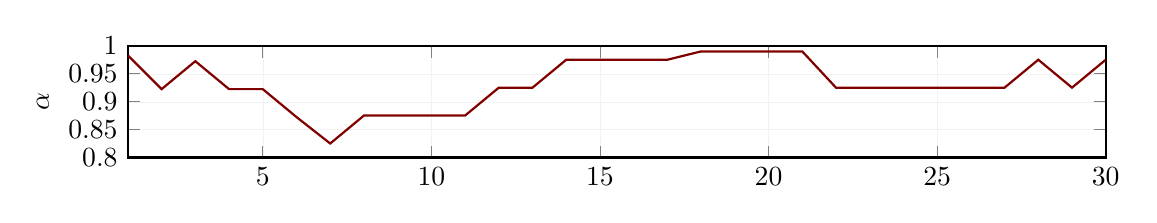
\begin{tikzpicture}
\begin{axis}[
yticklabel style={/pgf/number format/fixed},
ylabel={$\alpha$},
xmin=1, xmax=30,
ymin=0.8, ymax=1,
grid=both,
grid style={line width=.1pt, draw=gray!10},
width=14cm,height=3cm,
xtick={0,5,10,15,20,25,30},
ytick={0.8,0.85,0.9,0.95,1},
thick
]

\addplot[
color=Maroon
]
coordinates {
(1,0.982913070094558)(2,0.922441481135006)(3,0.972441481135006)(4,0.922441481135006)(5,0.922441481135006)(6,0.872441481135005)(7,0.825081107421489)(8,0.875081107421489)(9,0.875081107421489)(10,0.875081107421489)(11,0.875081107421489)(12,0.925081107421489)(13,0.925081107421489)(14,0.975081107421489)(15,0.975081107421489)(16,0.975081107421489)(17,0.975081107421489)(18,0.990000000000000)(19,0.990000000000000)(20,0.990000000000000)(21,0.990000000000000)(22,0.925081107421489)(23,0.925081107421489)(24,0.925081107421489)(25,0.925081107421489)(26,0.925081107421489)(27,0.925081107421489)(28,0.975081107421489)(29,0.925081107421489)(30,0.975081107421489)
};

\end{axis}
\end{tikzpicture}

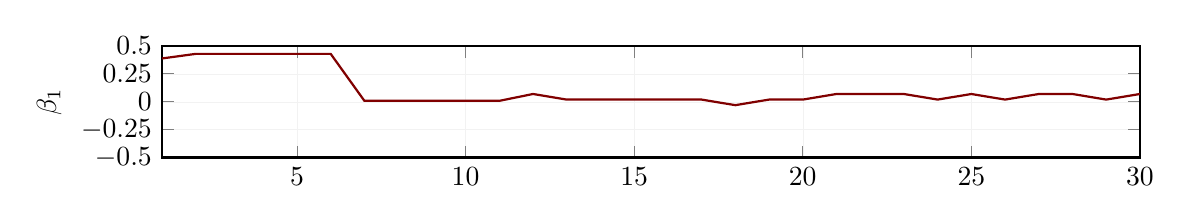
\begin{tikzpicture}
\begin{axis}[
yticklabel style={/pgf/number format/fixed},
ylabel={$\beta_1$},
xmin=1, xmax=30,
ymin=-0.5, ymax=0.5,
grid=both,
grid style={line width=.1pt, draw=gray!10},
width=14cm,height=3cm,
xtick={0,5,10,15,20,25,30},
ytick={-0.5,-0.25,0,0.25,0.5},
thick
]

\addplot[color=Maroon]
coordinates {
(1,0.386914402744206)(2,0.427964298417024)(3,0.427964298417024)(4,0.427964298417024)(5,0.427964298417024)(6,0.427964298417024)(7,0.00722167306420235)(8,0.00722167306420235)(9,0.00722167306420235)(10,0.00722167306420235)(11,0.00722167306420235)(12,0.0685452893600412)(13,0.0185452893600412)(14,0.0185452893600412)(15,0.0185452893600412)(16,0.0185452893600412)(17,0.0185452893600412)(18,-0.0314547106399588)(19,0.0185452893600412)(20,0.0185452893600412)(21,0.0685452893600412)(22,0.0685452893600412)(23,0.0685452893600412)(24,0.0185452893600412)(25,0.0685452893600412)(26,0.0185452893600412)(27,0.0685452893600412)(28,0.0685452893600412)(29,0.0185452893600412)(30,0.0685452893600412)
};
\end{axis}
\end{tikzpicture}

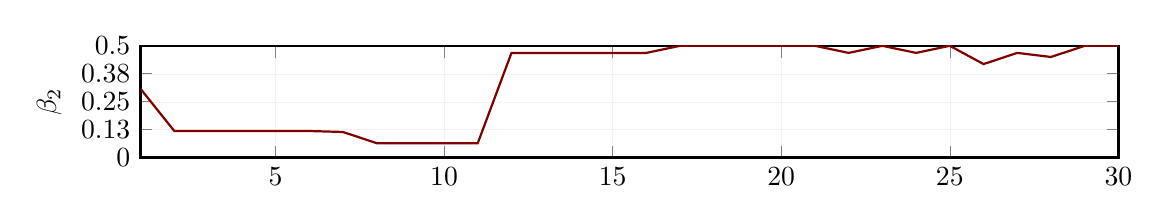
\begin{tikzpicture}
\begin{axis}[
yticklabel style={/pgf/number format/fixed},
ylabel={$\beta_2$},
xmin=1, xmax=30,
ymin=0, ymax=0.5,
grid=both,	      
scaled y ticks = false,		
grid style={line width=.1pt, draw=gray!10},
width=14cm,height=3cm,
xtick={0,5,10,15,20,25,30},
ytick={0,0.125,0.25,0.375,0.5},
thick
]

\addplot[color=Maroon]
coordinates {
(1,0.307368605261352)(2,0.118617020744079)(3,0.118617020744079)(4,0.118617020744079)(5,0.118617020744079)(6,0.118617020744079)(7,0.114290753138913)(8,0.0642907531389132)(9,0.0642907531389132)(10,0.0642907531389132)(11,0.0642907531389132)(12,0.468299759288352)(13,0.468299759288352)(14,0.468299759288352)(15,0.468299759288352)(16,0.468299759288352)(17,0.500000000000000)(18,0.500000000000000)(19,0.500000000000000)(20,0.500000000000000)(21,0.500000000000000)(22,0.468299759288352)(23,0.500000000000000)(24,0.468299759288352)(25,0.500000000000000)(26,0.418299759288352)(27,0.468299759288352)(28,0.450000000000000)(29,0.500000000000000)(30,0.500000000000000)
};
\end{axis}
\end{tikzpicture}
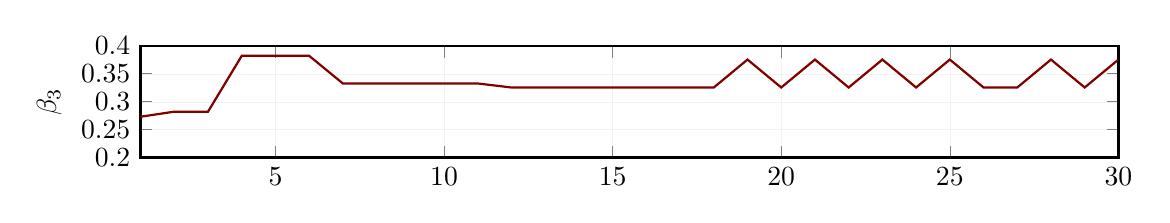
\begin{tikzpicture}
\begin{axis}[
yticklabel style={/pgf/number format/fixed},
ylabel={$\beta_3$},
xmin=1, xmax=30,
ymin=0.2, ymax=0.4,
grid=both,	      
scaled y ticks = false,		
grid style={line width=.1pt, draw=gray!10},
width=14cm,height=3cm,
xtick={0,5,10,15,20,25,30},
ytick={0.2,0.25,0.3,0.35,0.4},
thick
]

\addplot[color=Maroon]
coordinates {
(1,0.273026076343718)(2,0.282078656184312)(3,0.282078656184312)(4,0.382078656184312)(5,0.382078656184312)(6,0.382078656184312)(7,0.332560828042939)(8,0.332560828042939)(9,0.332560828042939)(10,0.332560828042939)(11,0.332560828042939)(12,0.325363152415932)(13,0.325363152415932)(14,0.325363152415932)(15,0.325363152415932)(16,0.325363152415932)(17,0.325363152415932)(18,0.325363152415932)(19,0.375363152415932)(20,0.325363152415932)(21,0.375363152415932)(22,0.325363152415932)(23,0.375363152415932)(24,0.325363152415932)(25,0.375363152415932)(26,0.325363152415932)(27,0.325363152415932)(28,0.375363152415932)(29,0.325363152415932)(30,0.375363152415932)
};
\end{axis}
\end{tikzpicture}
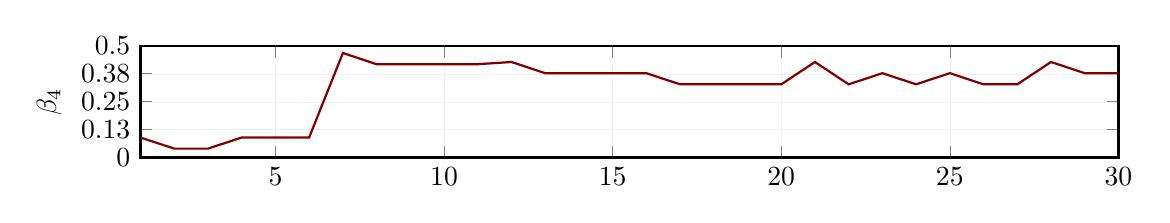
\begin{tikzpicture}
\begin{axis}[
yticklabel style={/pgf/number format/fixed},
ylabel={$\beta_4$},
xmin=1, xmax=30,
ymin=0, ymax=0.5,
grid=both,	      
scaled y ticks = false,		
grid style={line width=.1pt, draw=gray!10},
width=14cm,height=3cm,
xtick={0,5,10,15,20,25,30},
ytick={0,0.125,0.25,0.375,0.5},
thick
]

\addplot[color=Maroon]
coordinates {
	(1,0.0891652713175580)(2,0.0397335071068401)(3,0.0397335071068401)(4,0.0897335071068401)(5,0.0897335071068401)(6,0.0897335071068401)(7,0.467683658260978)(8,0.417683658260978)(9,0.417683658260978)(10,0.417683658260978)(11,0.417683658260978)(12,0.427535364587383)(13,0.377535364587383)(14,0.377535364587383)(15,0.377535364587383)(16,0.377535364587383)(17,0.327535364587383)(18,0.327535364587383)(19,0.327535364587383)(20,0.327535364587383)(21,0.427535364587383)(22,0.327535364587383)(23,0.377535364587383)(24,0.327535364587383)(25,0.377535364587383)(26,0.327535364587383)(27,0.327535364587383)(28,0.427535364587383)(29,0.377535364587383)(30,0.377535364587383)
};
\end{axis}
\end{tikzpicture}
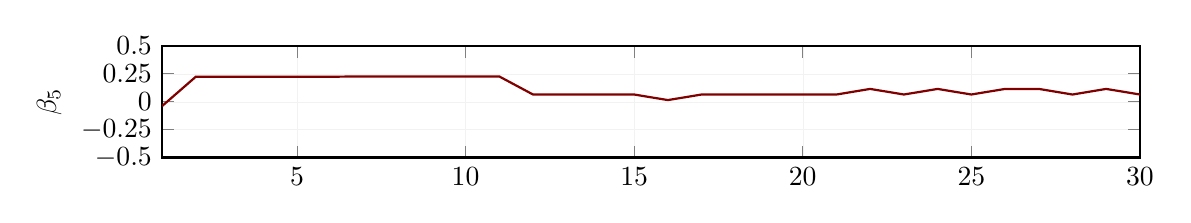
\begin{tikzpicture}
\begin{axis}[
yticklabel style={/pgf/number format/fixed},
ylabel={$\beta_5$},
xmin=1, xmax=30,
ymin=-0.5, ymax=0.5,
grid=both,	      
scaled y ticks = false,		
grid style={line width=.1pt, draw=gray!10},
width=14cm,height=3cm,
xtick={0,5,10,15,20,25,30},
ytick={-0.5,-0.25,0,0.25,0.5},
thick
]

\addplot[color=Maroon]
coordinates {
(1,-0.0393534392859444)(2,0.223391221365688)(3,0.223391221365688)(4,0.223391221365688)(5,0.223391221365688)(6,0.223391221365688)(7,0.225515923513374)(8,0.225515923513374)(9,0.225515923513374)(10,0.225515923513374)(11,0.225515923513374)(12,0.0640220444938637)(13,0.0640220444938637)(14,0.0640220444938637)(15,0.0640220444938637)(16,0.0140220444938637)(17,0.0640220444938637)(18,0.0640220444938637)(19,0.0640220444938637)(20,0.0640220444938637)(21,0.0640220444938637)(22,0.114022044493864)(23,0.0640220444938637)(24,0.114022044493864)(25,0.0640220444938637)(26,0.114022044493864)(27,0.114022044493864)(28,0.0640220444938637)(29,0.114022044493864)(30,0.0640220444938637)
};
\end{axis}
\end{tikzpicture}
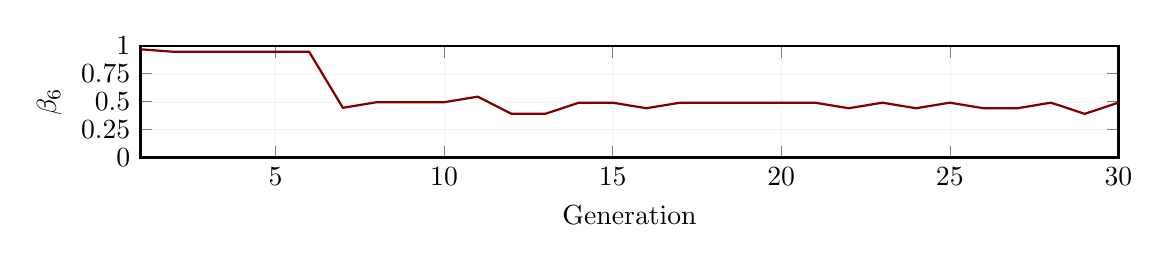
\begin{tikzpicture}
\begin{axis}[
yticklabel style={/pgf/number format/fixed},
xlabel={Generation},
ylabel={$\beta_6$},
xmin=1, xmax=30,
ymin=0, ymax=1,
grid=both,	      
scaled y ticks = false,		
grid style={line width=.1pt, draw=gray!10},
width=14cm,height=3cm,
xtick={0,5,10,15,20,25,30},
ytick={0,0.25,0.5,0.75,1},
thick
]

\addplot[color=Maroon]
coordinates {
(1,0.968838961699090)(2,0.946212413407763)(3,0.946212413407763)(4,0.946212413407763)(5,0.946212413407763)(6,0.946212413407763)(7,0.444870432050475)(8,0.494870432050475)(9,0.494870432050475)(10,0.494870432050475)(11,0.544870432050475)(12,0.390908636004713)(13,0.390908636004713)(14,0.490908636004713)(15,0.490908636004713)(16,0.440908636004713)(17,0.490908636004713)(18,0.490908636004713)(19,0.490908636004713)(20,0.490908636004713)(21,0.490908636004713)(22,0.440908636004713)(23,0.490908636004713)(24,0.440908636004713)(25,0.490908636004713)(26,0.440908636004713)(27,0.440908636004713)(28,0.490908636004713)(29,0.390908636004713)(30,0.490908636004713)
};
\end{axis}
\end{tikzpicture}
\caption{Genetic Algorithm -- Generalized Bouc-Wen Model (Random crossover)}
\label{fig:ga_gen_rand}
\end{figure}

The final values found for each parameter using the Genetic Algorithm approach
with the random crossover strategy are displayed in Table~\ref{tab:ga_gen_values_r}.


\begin{table}[H]
\centering
\begin{tabular}{l c c c c c c c c}
	\toprule
	\textbf{Parameter}		& $A$		& $\alpha$	& $\beta_1$	& $\beta_2$ & $\beta_3$	& $\beta_4$ & $\beta_5$ & $\beta_6$		\\ \midrule
	\textbf{Final value}	& $0.1$	& $0.9750$	& $0.0685$ & $0.5$ & $0.3753$	& $0.3775$	& $0.0640$	& $0.4909$	\\
	\bottomrule
\end{tabular}
\caption{Random Crossover -- Final values (Generalized Bouc-Wen model)}
\label{tab:ga_gen_values_r}
\end{table}


% weighted crossover - generalized bw model
\begin{figure}[H]
	\centering
	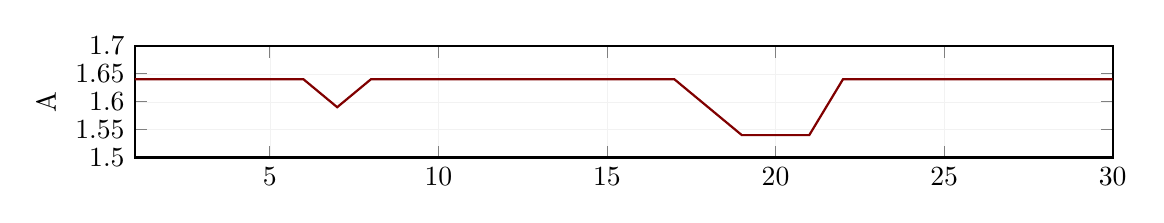
\begin{tikzpicture}
	\begin{axis}[
	yticklabel style={/pgf/number format/fixed},	
	ylabel={A},
	xmin=1, xmax=30,
	ymin=1.5, ymax=1.7,
	grid=both,
	grid style={line width=.1pt, draw=gray!10},
	width=14cm,height=3cm,
	xtick={0,5,10,15,20,25,30},
	ytick={1.5,1.55,1.6,1.65,1.7},
	thick]
	\addplot[color=Maroon]
	coordinates {
(1,1.64009787169959)(2,1.64009787169959)(3,1.64009787169959)(4,1.64009787169959)(5,1.64009787169959)(6,1.64009787169959)(7,1.59009787169959)(8,1.64009787169959)(9,1.64009787169959)(10,1.64009787169959)(11,1.64009787169959)(12,1.64009787169959)(13,1.64009787169959)(14,1.64009787169959)(15,1.64009787169959)(16,1.64009787169959)(17,1.64009787169959)(18,1.59009787169959)(19,1.54009787169959)(20,1.54009787169959)(21,1.54009787169959)(22,1.64009787169959)(23,1.64009787169959)(24,1.64009787169959)(25,1.64009787169959)(26,1.64009787169959)(27,1.64009787169959)(28,1.64009787169959)(29,1.64009787169959)(30,1.64009787169959)
	};
	\end{axis}
	\end{tikzpicture}
	
	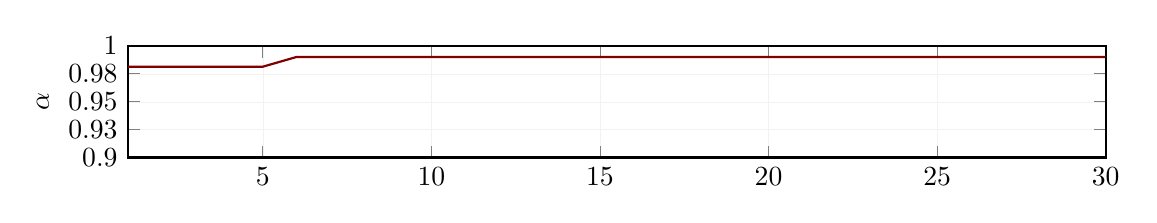
\begin{tikzpicture}
	\begin{axis}[
	yticklabel style={/pgf/number format/fixed},
	ylabel={$\alpha$},
	xmin=1, xmax=30,
	ymin=0.9, ymax=1,
	grid=both,
	grid style={line width=.1pt, draw=gray!10},
	width=14cm,height=3cm,
	xtick={0,5,10,15,20,25,30},
	ytick={0.9,0.925,0.95,0.975,1},
	thick
	]
	
	\addplot[
	color=Maroon
	]
	coordinates {
(1,0.981296401853448)(2,0.981296401853448)(3,0.981296401853448)(4,0.981296401853448)(5,0.981296401853448)(6,0.990000000000000)(7,0.990000000000000)(8,0.990000000000000)(9,0.990000000000000)(10,0.990000000000000)(11,0.990000000000000)(12,0.990000000000000)(13,0.990000000000000)(14,0.990000000000000)(15,0.990000000000000)(16,0.990000000000000)(17,0.990000000000000)(18,0.990000000000000)(19,0.990000000000000)(20,0.990000000000000)(21,0.990000000000000)(22,0.990000000000000)(23,0.990000000000000)(24,0.990000000000000)(25,0.990000000000000)(26,0.990000000000000)(27,0.990000000000000)(28,0.990000000000000)(29,0.990000000000000)(30,0.990000000000000)
	};
	
	\end{axis}
	\end{tikzpicture}
	
	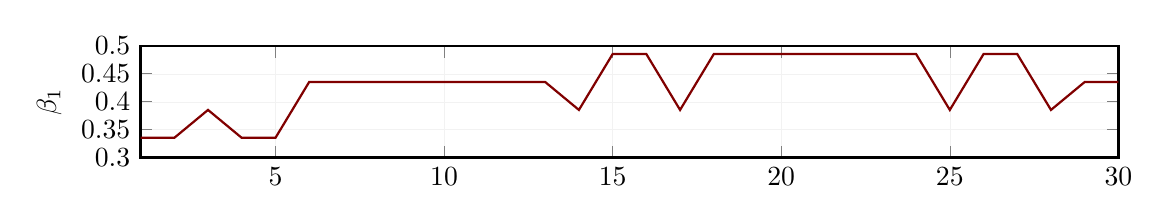
\begin{tikzpicture}
	\begin{axis}[
	yticklabel style={/pgf/number format/fixed},
	ylabel={$\beta_1$},
	xmin=1, xmax=30,
	ymin=0.3, ymax=0.5,
	grid=both,
	grid style={line width=.1pt, draw=gray!10},
	width=14cm,height=3cm,
	xtick={0,5,10,15,20,25,30},
	ytick={0.3,0.35,0.4,0.45,0.5},
	thick
	]
	
	\addplot[color=Maroon]
	coordinates {
(1,0.335200906831924)(2,0.335200906831924)(3,0.385200906831924)(4,0.335200906831924)(5,0.335200906831924)(6,0.435200906831924)(7,0.435200906831924)(8,0.435200906831924)(9,0.435200906831924)(10,0.435200906831924)(11,0.435200906831924)(12,0.435200906831924)(13,0.435200906831924)(14,0.385200906831924)(15,0.485200906831924)(16,0.485200906831924)(17,0.385200906831924)(18,0.485200906831924)(19,0.485200906831924)(20,0.485200906831924)(21,0.485200906831924)(22,0.485200906831924)(23,0.485200906831924)(24,0.485200906831924)(25,0.385200906831924)(26,0.485200906831924)(27,0.485200906831924)(28,0.385200906831924)(29,0.435200906831924)(30,0.435200906831924)
	};
	\end{axis}
	\end{tikzpicture}
	
	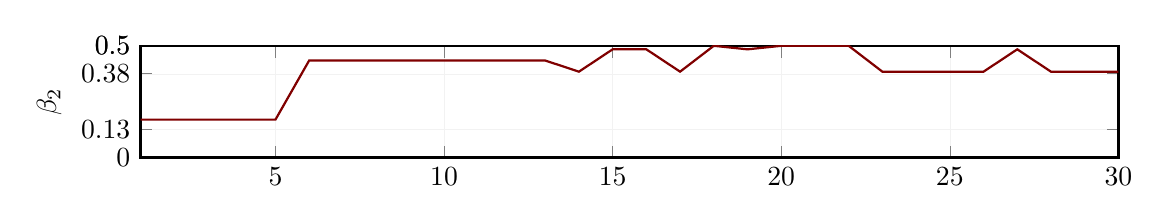
\begin{tikzpicture}
	\begin{axis}[
	yticklabel style={/pgf/number format/fixed},
	ylabel={$\beta_2$},
	xmin=1, xmax=30,
	ymin=0, ymax=0.5,
	grid=both,	      
	scaled y ticks = false,		
	grid style={line width=.1pt, draw=gray!10},
	width=14cm,height=3cm,
	xtick={0,5,10,15,20,25,30},
	ytick={0,0.125,0.5,0.375,0.5},
	thick
	]
	
	\addplot[color=Maroon]
	coordinates {
(1,0.169549755213670)(2,0.169549755213670)(3,0.169549755213670)(4,0.169549755213670)(5,0.169549755213670)(6,0.434227178406584)(7,0.434227178406584)(8,0.434227178406584)(9,0.434227178406584)(10,0.434227178406584)(11,0.434227178406584)(12,0.434227178406584)(13,0.434227178406584)(14,0.384227178406584)(15,0.484227178406584)(16,0.484227178406584)(17,0.384227178406584)(18,0.500000000000000)(19,0.484227178406584)(20,0.500000000000000)(21,0.500000000000000)(22,0.500000000000000)(23,0.384227178406584)(24,0.384227178406584)(25,0.384227178406584)(26,0.384227178406584)(27,0.484227178406584)(28,0.384227178406584)(29,0.384227178406584)(30,0.384227178406584)
	};
	\end{axis}
	\end{tikzpicture}
	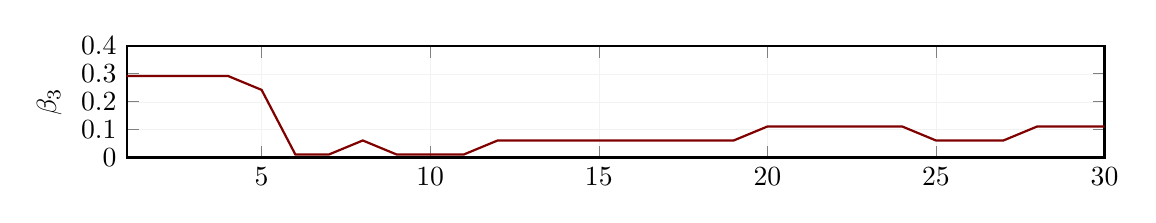
\begin{tikzpicture}
	\begin{axis}[
	yticklabel style={/pgf/number format/fixed},
	ylabel={$\beta_3$},
	xmin=1, xmax=30,
	ymin=0, ymax=0.4,
	grid=both,	      
	scaled y ticks = false,		
	grid style={line width=.1pt, draw=gray!10},
	width=14cm,height=3cm,
	xtick={0,5,10,15,20,25,30},
	ytick={0,0.1,0.2,0.3,0.4},
	thick
	]
	
	\addplot[color=Maroon]
	coordinates {
(1,0.292135220884937)(2,0.292135220884937)(3,0.292135220884937)(4,0.292135220884937)(5,0.242135220884937)(6,0.0109556696552213)(7,0.0109556696552213)(8,0.0609556696552213)(9,0.0109556696552213)(10,0.0109556696552213)(11,0.0109556696552213)(12,0.0609556696552213)(13,0.0609556696552213)(14,0.0609556696552213)(15,0.0609556696552213)(16,0.0609556696552213)(17,0.0609556696552213)(18,0.0609556696552213)(19,0.0609556696552213)(20,0.110955669655221)(21,0.110955669655221)(22,0.110955669655221)(23,0.110955669655221)(24,0.110955669655221)(25,0.0609556696552213)(26,0.0609556696552213)(27,0.0609556696552213)(28,0.110955669655221)(29,0.110955669655221)(30,0.110955669655221)
	};
	\end{axis}
	\end{tikzpicture}
	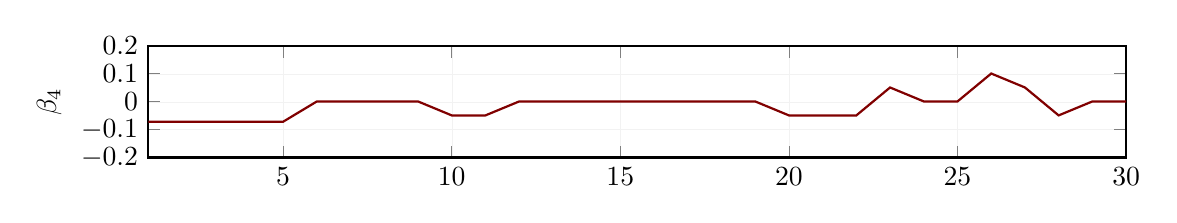
\begin{tikzpicture}
	\begin{axis}[
	yticklabel style={/pgf/number format/fixed},
	ylabel={$\beta_4$},
	xmin=1, xmax=30,
	ymin=-0.2, ymax=0.2,
	grid=both,	      
	scaled y ticks = false,		
	grid style={line width=.1pt, draw=gray!10},
	width=14cm,height=3cm,
	xtick={0,5,10,15,20,25,30},
	ytick={-0.2,-0.1,0,0.1,0.2},
	thick
	]
	
	\addplot[color=Maroon]
	coordinates {
(1,-0.0718640159281633)(2,-0.0718640159281633)(3,-0.0718640159281633)(4,-0.0718640159281633)(5,-0.0718640159281633)(6,0.000777359931312296)(7,0.000777359931312296)(8,0.000777359931312296)(9,0.000777359931312296)(10,-0.0492226400686877)(11,-0.0492226400686877)(12,0.000777359931312296)(13,0.000777359931312296)(14,0.000777359931312296)(15,0.000777359931312296)(16,0.000777359931312296)(17,0.000777359931312296)(18,0.000777359931312296)(19,0.000777359931312296)(20,-0.0492226400686877)(21,-0.0492226400686877)(22,-0.0492226400686877)(23,0.0507773599313123)(24,0.000777359931312296)(25,0.000777359931312296)(26,0.100777359931312)(27,0.0507773599313123)(28,-0.0492226400686877)(29,0.000777359931312296)(30,0.000777359931312296)
	};
	\end{axis}
	\end{tikzpicture}
	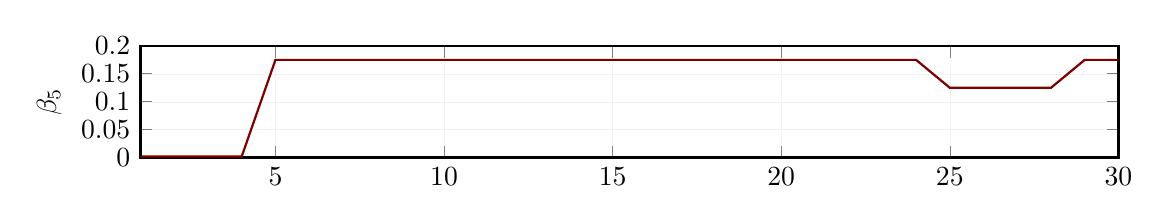
\begin{tikzpicture}
	\begin{axis}[
	yticklabel style={/pgf/number format/fixed},
	ylabel={$\beta_5$},
	xmin=1, xmax=30,
	ymin=0, ymax=0.2,
	grid=both,	      
	scaled y ticks = false,		
	grid style={line width=.1pt, draw=gray!10},
	width=14cm,height=3cm,
	xtick={0,5,10,15,20,25,30},
	ytick={0,0.05,0.1,0.15,0.2},
	thick
	]
	
	\addplot[color=Maroon]
	coordinates {
(1,0.00194303788602943)(2,0.00194303788602943)(3,0.00194303788602943)(4,0.00194303788602943)(5,0.174821464405275)(6,0.174821464405275)(7,0.174821464405275)(8,0.174821464405275)(9,0.174821464405275)(10,0.174821464405275)(11,0.174821464405275)(12,0.174821464405275)(13,0.174821464405275)(14,0.174821464405275)(15,0.174821464405275)(16,0.174821464405275)(17,0.174821464405275)(18,0.174821464405275)(19,0.174821464405275)(20,0.174821464405275)(21,0.174821464405275)(22,0.174821464405275)(23,0.174821464405275)(24,0.174821464405275)(25,0.124821464405275)(26,0.124821464405275)(27,0.124821464405275)(28,0.124821464405275)(29,0.174821464405275)(30,0.174821464405275)
	};
	\end{axis}
	\end{tikzpicture}
	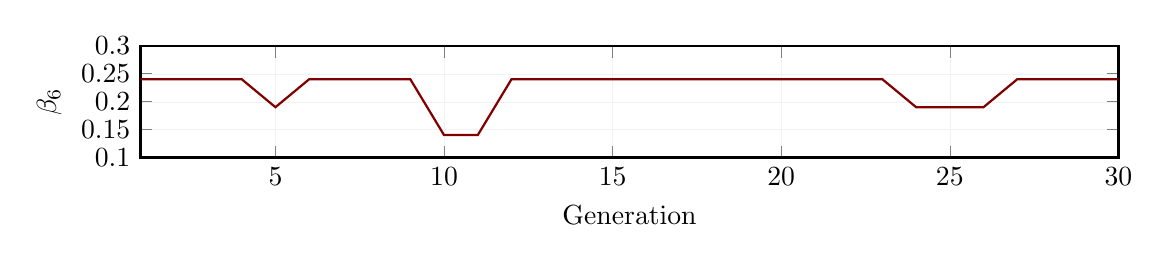
\begin{tikzpicture}
	\begin{axis}[
	yticklabel style={/pgf/number format/fixed},
	xlabel={Generation},
	ylabel={$\beta_6$},
	xmin=1, xmax=30,
	ymin=0.1, ymax=0.3,
	grid=both,	      
	scaled y ticks = false,		
	grid style={line width=.1pt, draw=gray!10},
	width=14cm,height=3cm,
	xtick={0,5,10,15,20,25,30},
	ytick={0.1,0.15,0.2,0.25,0.3},
	thick
	]
	
	\addplot[color=Maroon]
	coordinates {
(1,0.240120322494038)(2,0.240120322494038)(3,0.240120322494038)(4,0.240120322494038)(5,0.190120322494038)(6,0.240120322494038)(7,0.240120322494038)(8,0.240120322494038)(9,0.240120322494038)(10,0.140120322494038)(11,0.140120322494038)(12,0.240120322494038)(13,0.240120322494038)(14,0.240120322494038)(15,0.240120322494038)(16,0.240120322494038)(17,0.240120322494038)(18,0.240120322494038)(19,0.240120322494038)(20,0.240120322494038)(21,0.240120322494038)(22,0.240120322494038)(23,0.240120322494038)(24,0.190120322494038)(25,0.190120322494038)(26,0.190120322494038)(27,0.240120322494038)(28,0.240120322494038)(29,0.240120322494038)(30,0.240120322494038)
	};
	\end{axis}
	\end{tikzpicture}
	\caption{Genetic Algorithm -- Generalized Bouc-Wen Model (Weighted crossover)}
	\label{fig:ga_gen_w}
\end{figure}

The final values found for each parameter using the Genetic Algorithm approach
with the weighted crossover strategy are displayed in Table~\ref{tab:ga_gen_final_w}.


\begin{table}[H]
	\centering
	\begin{tabular}{l c c c c c c c c}
		\toprule
		\textbf{Parameter}		& $A$		& $\alpha$	& $\beta_1$	& $\beta_2$ & $\beta_3$	& $\beta_4$ & $\beta_5$ & $\beta_6$		\\ \midrule
		\textbf{Final value}	& $1.6401$	& $0.99$	& $0.4352$ & $0.3842$ & $0.1110$	& $0.0007$	& $0.1748$	& $0.2401$	\\
		\bottomrule
	\end{tabular}
	\caption{Weighted Crossover -- Final values (Generalized Bouc-Wen model)}
	\label{tab:ga_gen_final_w}
\end{table}


% proportional crossover - generalized bw model
\begin{figure}[H]
	\centering
	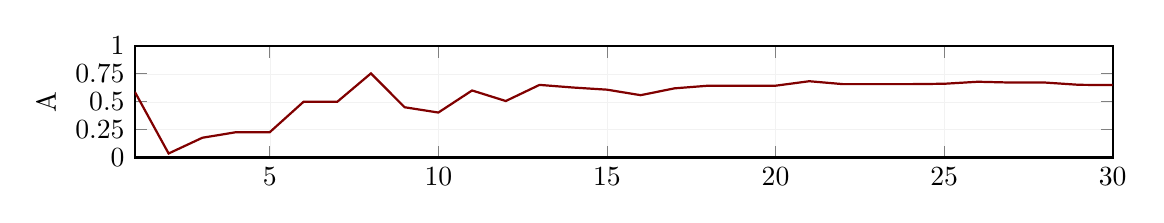
\begin{tikzpicture}
	\begin{axis}[
	yticklabel style={/pgf/number format/fixed},	
	ylabel={A},
	xmin=1, xmax=30,
	ymin=0, ymax=1,
	grid=both,
	grid style={line width=.1pt, draw=gray!10},
	width=14cm,height=3cm,
	xtick={0,5,10,15,20,25,30},
	ytick={0,0.25,0.5,0.75,1},
	thick]
	\addplot[color=Maroon]
	coordinates {
(1,0.586789085025302)(2,0.0358967562890904)(3,0.176681141073827)(4,0.226681141073827)(5,0.226681141073827)(6,0.498384582712587)(7,0.498384582712587)(8,0.752873226193916)(9,0.449887946483127)(10,0.402546078770074)(11,0.600134245317030)(12,0.505770155753776)(13,0.650134245317030)(14,0.626394823971145)(15,0.607372852387976)(16,0.557936687198418)(17,0.619085169511363)(18,0.642805105513447)(19,0.642805105513447)(20,0.642805105513447)(21,0.682916787238431)(22,0.656879509464287)(23,0.656879509464287)(24,0.656879509464287)(25,0.660121724504005)(26,0.678221309937812)(27,0.670896376330679)(28,0.670896376330679)(29,0.650698320273573)(30,0.648436342261247)
	};
	\end{axis}
	\end{tikzpicture}
	
	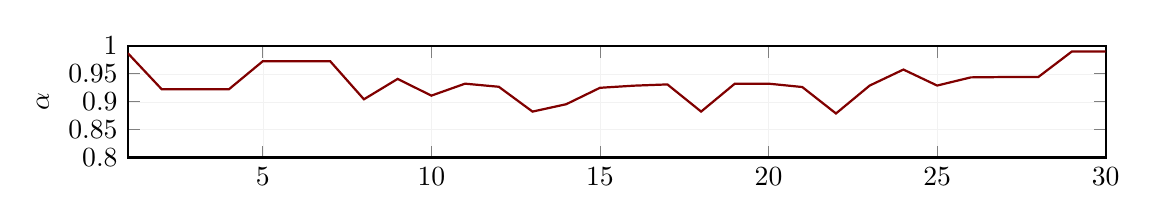
\begin{tikzpicture}
	\begin{axis}[
	yticklabel style={/pgf/number format/fixed},
	ylabel={$\alpha$},
	xmin=1, xmax=30,
	ymin=0.8, ymax=1,
	grid=both,
	grid style={line width=.1pt, draw=gray!10},
	width=14cm,height=3cm,
	xtick={0,5,10,15,20,25,30},
	ytick={0.8,0.85,0.9,0.95,1},
	thick
	]
	
	\addplot[
	color=Maroon
	]
	coordinates {
(1,0.986672283249516)(2,0.922382834644631)(3,0.922382834644631)(4,0.922382834644631)(5,0.972382834644631)(6,0.972382834644631)(7,0.972382834644631)(8,0.904239327301436)(9,0.940741403341614)(10,0.910797043828711)(11,0.932215557670407)(12,0.926649119672661)(13,0.882215557670407)(14,0.895428156016643)(15,0.924812943367856)(16,0.928617651796015)(17,0.930869249870665)(18,0.882215557670407)(19,0.932215557670407)(20,0.932215557670407)(21,0.926195919865785)(22,0.878837180255882)(23,0.928837180255882)(24,0.957482403154262)(25,0.928837180255882)(26,0.943482841695566)(27,0.944091666776735)(28,0.944091666776735)(29,0.990000000000000)(30,0.990000000000000)
	};
	
	\end{axis}
	\end{tikzpicture}
	
	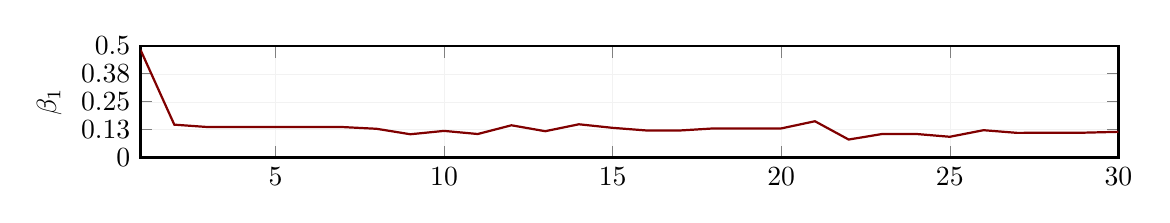
\begin{tikzpicture}
	\begin{axis}[
	yticklabel style={/pgf/number format/fixed},
	ylabel={$\beta_1$},
	xmin=1, xmax=30,
	ymin=0, ymax=0.5,
	grid=both,
	grid style={line width=.1pt, draw=gray!10},
	width=14cm,height=3cm,
	xtick={0,5,10,15,20,25,30},
	ytick={0,0.125,0.25,0.375,0.5},
	thick
	]
	
	\addplot[color=Maroon]
	coordinates {
(1,0.481372800365983)(2,0.147069795573228)(3,0.136260718301767)(4,0.136260718301767)(5,0.136260718301767)(6,0.136260718301767)(7,0.136260718301767)(8,0.128537139120550)(9,0.104097511498838)(10,0.119098283862123)(11,0.105177371117901)(12,0.144236883850152)(13,0.117738308344768)(14,0.148746149355357)(15,0.132795682152641)(16,0.121056019994579)(17,0.121008726058946)(18,0.130190517812153)(19,0.130190517812153)(20,0.130190517812153)(21,0.162316355897392)(22,0.0803979620655346)(23,0.105399371388921)(24,0.105399371388921)(25,0.0927992179601150)(26,0.122258455901548)(27,0.110217127205781)(28,0.110850745567709)(29,0.111216901386996)(30,0.114921697740118)
	};
	\end{axis}
	\end{tikzpicture}
	
	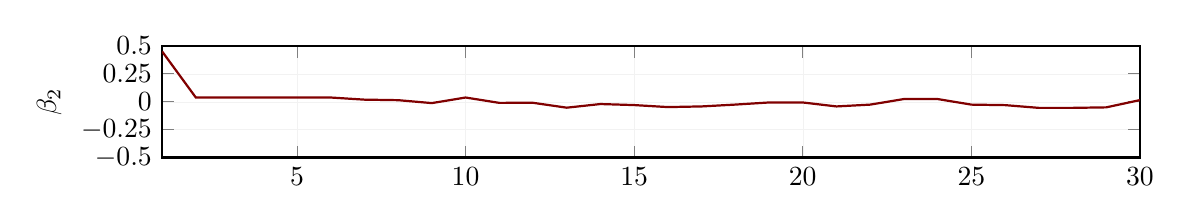
\begin{tikzpicture}
	\begin{axis}[
	yticklabel style={/pgf/number format/fixed},
	ylabel={$\beta_2$},
	xmin=1, xmax=30,
	ymin=-0.5, ymax=0.5,
	grid=both,	      
	scaled y ticks = false,		
	grid style={line width=.1pt, draw=gray!10},
	width=14cm,height=3cm,
	xtick={0,5,10,15,20,25,30},
	ytick={-0.5,-0.25,0,0.25,0.5},
	thick
	]
	
	\addplot[color=Maroon]
	coordinates {
(1,0.449916635667667)(2,0.0370768904468451)(3,0.0370768904468451)(4,0.0370768904468451)(5,0.0370768904468451)(6,0.0370768904468451)(7,0.0179811950636510)(8,0.0132517273186676)(9,-0.0129231095531549)(10,0.0370768904468451)(11,-0.0108671354937760)(12,-0.0102798748077285)(13,-0.0539189350355483)(14,-0.0212844051124743)(15,-0.0305969352720136)(16,-0.0486038760470906)(17,-0.0427156579064975)(18,-0.0262723796864142)(19,-0.00727762163018886)(20,-0.00727762163018886)(21,-0.0427285137498147)(22,-0.0265966897159562)(23,0.0234033102840438)(24,0.0234033102840438)(25,-0.0265966897159562)(26,-0.0310932226671911)(27,-0.0556519361527456)(28,-0.0556519361527456)(29,-0.0510474099686665)(30,0.0139143390935065)
	};
	\end{axis}
	\end{tikzpicture}
		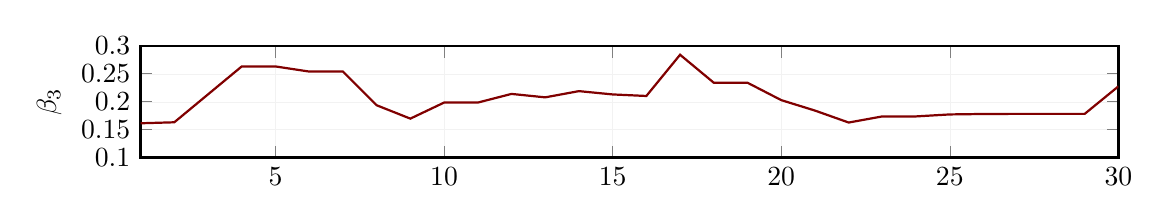
\begin{tikzpicture}
	\begin{axis}[
	yticklabel style={/pgf/number format/fixed},
	ylabel={$\beta_3$},
	xmin=1, xmax=30,
	ymin=0.1, ymax=0.3,
	grid=both,	      
	scaled y ticks = false,		
	grid style={line width=.1pt, draw=gray!10},
	width=14cm,height=3cm,
	xtick={0,5,10,15,20,25,30},
	ytick={0.1,0.15,0.2,0.25,0.3},
	thick
	]
	
	\addplot[color=Maroon]
	coordinates {
(1,0.161287143982303)(2,0.163062339392973)(3,0.213062339392973)(4,0.263062339392973)(5,0.263062339392973)(6,0.253902401387567)(7,0.253902401387567)(8,0.193606495353288)(9,0.169613129076818)(10,0.198322996529753)(11,0.198322996529753)(12,0.213875635945515)(13,0.207719095346517)(14,0.218852076837020)(15,0.212940684760854)(16,0.210169984852480)(17,0.284008343544958)(18,0.233880090278388)(19,0.233880090278388)(20,0.202760931297712)(21,0.184048212153045)(22,0.162631219662305)(23,0.173605174605402)(24,0.173605174605402)(25,0.177130106904538)(26,0.177942256892546)(27,0.178148074457517)(28,0.178148074457517)(29,0.178148074457517)(30,0.227407354518908)
	};
	\end{axis}
	\end{tikzpicture}
	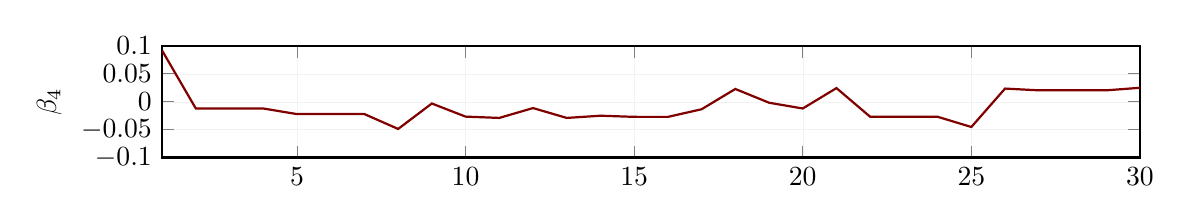
\begin{tikzpicture}
	\begin{axis}[
	yticklabel style={/pgf/number format/fixed},
	ylabel={$\beta_4$},
	xmin=1, xmax=30,
	ymin=-0.1, ymax=0.1,
	grid=both,	      
	scaled y ticks = false,		
	grid style={line width=.1pt, draw=gray!10},
	width=14cm,height=3cm,
	xtick={0,5,10,15,20,25,30},
	ytick={-0.1,-0.05,0,0.05,0.1},
	thick
	]
	
	\addplot[color=Maroon]
	coordinates {
(1,0.0915330239914958)(2,-0.0122462477359733)(3,-0.0122462477359733)(4,-0.0122462477359733)(5,-0.0222613398910149)(6,-0.0222613398910149)(7,-0.0222613398910149)(8,-0.0488508504217125)(9,-0.00330106976743263)(10,-0.0267986032634243)(11,-0.0291235113607312)(12,-0.0114872011158797)(13,-0.0291235113607312)(14,-0.0251777415071699)(15,-0.0272074498192450)(16,-0.0272710184385404)(17,-0.0135955716171374)(18,0.0227289815614596)(19,-0.00189683988997794)(20,-0.0122375270670718)(21,0.0242856889792331)(22,-0.0270973777919590)(23,-0.0270973777919590)(24,-0.0270973777919590)(25,-0.0453666985431060)(26,0.0234238633158912)(27,0.0202741057465342)(28,0.0202740149828679)(29,0.0202739625322973)(30,0.0248547187303980)
	};
	\end{axis}
	\end{tikzpicture}
		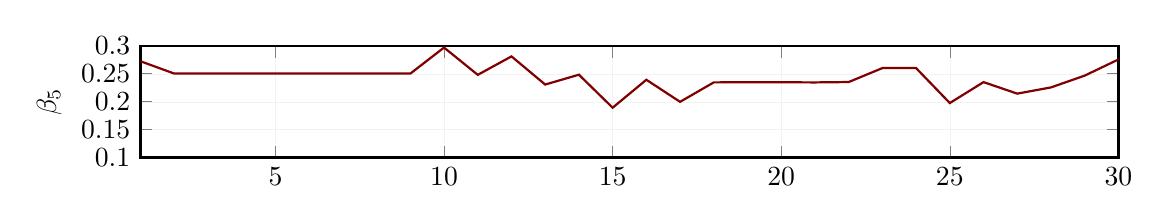
\begin{tikzpicture}
	\begin{axis}[
	yticklabel style={/pgf/number format/fixed},
	ylabel={$\beta_5$},
	xmin=1, xmax=30,
	ymin=0.1, ymax=0.3,
	grid=both,	      
	scaled y ticks = false,		
	grid style={line width=.1pt, draw=gray!10},
	width=14cm,height=3cm,
	xtick={0,5,10,15,20,25,30},
	ytick={0.1,0.15,0.2,0.25,0.3},
	thick
	]
	
	\addplot[color=Maroon]
	coordinates {
(1,0.272258898620322)(2,0.250257903080575)(3,0.250257903080575)(4,0.250257903080575)(5,0.250257903080575)(6,0.250257903080575)(7,0.250257903080575)(8,0.250257903080575)(9,0.250257903080575)(10,0.296889604644051)(11,0.248012550513676)(12,0.281067749871438)(13,0.230640106493696)(14,0.248268645200886)(15,0.189200445024400)(16,0.239203703439200)(17,0.199691934816109)(18,0.234526058412463)(19,0.234719180387835)(20,0.234719180387835)(21,0.234467563113400)(22,0.235133184343071)(23,0.260080534096181)(24,0.260080534096181)(25,0.197507625486695)(26,0.235002983494812)(27,0.214375305160957)(28,0.225515678611458)(29,0.246621699159725)(30,0.275515678611458)
	};
	\end{axis}
	\end{tikzpicture}
		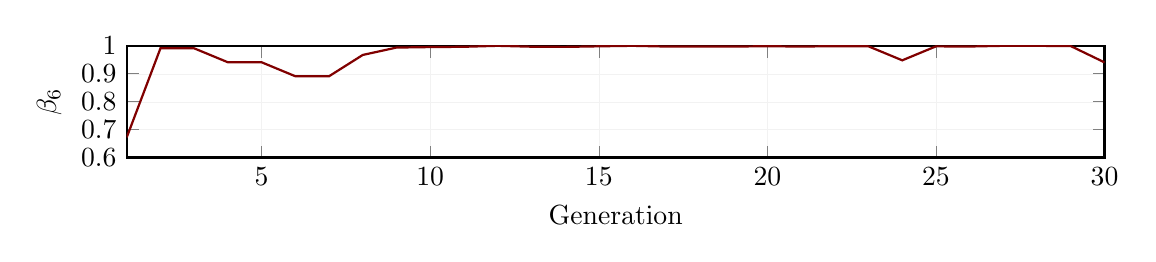
\begin{tikzpicture}
	\begin{axis}[
	yticklabel style={/pgf/number format/fixed},
	xlabel={Generation},
	ylabel={$\beta_6$},
	xmin=1, xmax=30,
	ymin=0.6, ymax=1,
	grid=both,	      
	scaled y ticks = false,		
	grid style={line width=.1pt, draw=gray!10},
	width=14cm,height=3cm,
	xtick={0,5,10,15,20,25,30},
	ytick={0.6,0.7,0.8,0.9,1},
	thick
	]
	
	\addplot[color=Maroon]
	coordinates {
(1,0.672149142917568)(2,0.991003314089209)(3,0.991003314089209)(4,0.941003314089209)(5,0.941003314089209)(6,0.891003314089209)(7,0.891003314089209)(8,0.967302642542328)(9,0.993731174347446)(10,0.995484463686964)(11,0.996522717662297)(12,1)(13,0.996850477831198)(14,0.996162800454658)(15,0.998213845691092)(16,1)(17,0.997429483805097)(18,0.997466188251416)(19,0.997466188251416)(20,0.998501496294619)(21,0.997423784085688)(22,0.998658849148204)(23,0.998046374827855)(24,0.948046374827855)(25,0.998059459387019)(26,0.997501603002940)(27,1)(28,1)(29,0.998927113840961)(30,0.940570170219691)
	};
	\end{axis}
	\end{tikzpicture}
	\caption{Genetic Algorithm -- Generalized Bouc-Wen Model (Proportional crossover)}
	\label{fig:ga_gen_prop}
\end{figure}

The final values found for each parameter using the Genetic Algorithm approach
with the proportional crossover strategy are displayed in Table~\ref{tab:ga_gen_values}.


\begin{table}[H]
	\centering
	\begin{tabular}{l c c c c c c c c}
		\toprule
		\textbf{Parameter}		& $A$		& $\alpha$	& $\beta_1$	& $\beta_2$ & $\beta_3$	& $\beta_4$ & $\beta_5$ & $\beta_6$		\\ \midrule
		\textbf{Final value}	& $0.6484$	& $0.99$	& $0.1149$ & $0.0139$ & $0.2274$	& $0.0248$	& $0.2755$	& $0.9405$	\\
		\bottomrule
	\end{tabular}
	\caption{Proportional Crossover -- Final values (Generalized Bouc-Wen model)}
	\label{tab:ga_gen_values}
\end{table}

As for the classic version of the Bouc-Wen model, it is possible to observe
that for the random and weighted crossover strategies the individuals' chromosomes
tend to sharply change between one value and another, as the set of possible values
is that of the first generation~\footnote{
Apart from eventual changes introduced by the mutation step at each generation.}.
In fact, the proportional crossover strategy figures a smoother trend for all variables.

Figure~\ref{fig:ga_gen_hys} shows how the hysteresis loop behaves using the final parameters of Table~\ref{tab:ga_gen_values}.
With respect to Figure~\ref{fig:ga_classic_res}, a higher precision is appreciable
thanks to the usage of the generalized hysteresis model.

\begin{figure}[H]
	\centering
	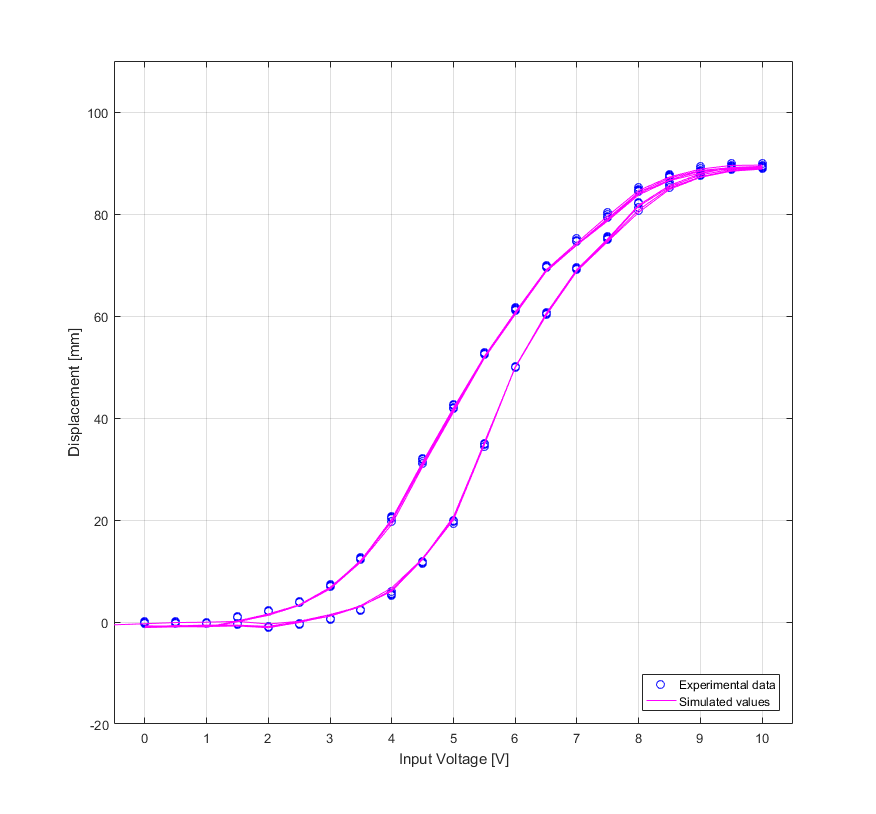
\includegraphics[width=\linewidth]{Images/ga_general_prop}
	\caption{Hysteresis loop result -- Genetic Algorithm's parameters (generalized Bouc-Wen model, proportional crossover approach)}
	\label{fig:ga_gen_hys}
\end{figure}

\subsubsection{Modified Firefly Algorithm -- Generalized Bouc-Wen Model}

Table~\ref{tab:mfa_gen_params} contains the parameters used for the
Modified Firefly Algorithm approach. 

\begin{table}[H]
	\centering
	\begin{tabular}{c c}
		\toprule
		\textbf{Parameter} & \textbf{Value} \\ \toprule
		$N$			& $10$ \\
		$G$			& $30$ \\
		$d$			& $8$  \\
		$L$			& $\left[0, 0.7, -0.1, -0.1, -0.1, -0.1, -0.1, -0.1\right]$ \\
		$U$			& $\left[1.5, 1, 0.5, 0.5, 0.5, 0.5, 0.5, 0.5\right]$ \\ 
		$a$			& $1.1$ \\
		$b$			& $0.3$ \\ \bottomrule
	\end{tabular}
	\caption{Parameters for the Modified Firefly Algorithm approach -- Generalized Bouc-Wen model}
	\label{tab:mfa_gen_params}
\end{table}

Figure~\ref{fig:mfa_gen_trend} shows the trend of generalized Bouc-Wen model
parameters using the Modified Firefly Algorithm. The value of the best firefly
for the specific generation is reported as the value outputted by the algorithm
for that generation.

It is also noticeable how the values initially tend to vary a lot,
as the fireflies broadly explore the solution space during the first generations,
and then proceed to refine the search around the fireflies
with highest lightness factor (local exploitation).

The hysteresis loop behaviour with the final parameters
is displayed in Figure~\ref{fig:mfa_gen_hys}.

\begin{figure}[H]
	\centering
	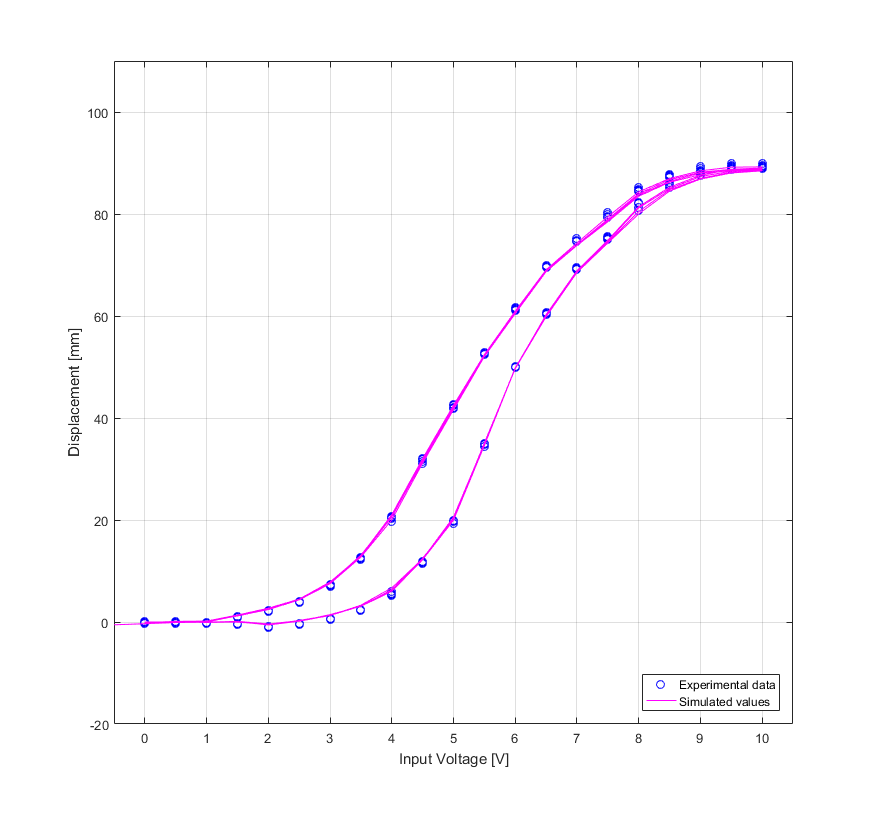
\includegraphics[width=0.9\linewidth]{Images/mfa_gen_final}
	\caption{Hysteresis loop result using Modified Firefly's parameters (generalized Bouc-Wen model)}
	\label{fig:mfa_gen_hys}
\end{figure}


% MFA generalized trend
\begin{figure}[H]
	\centering
	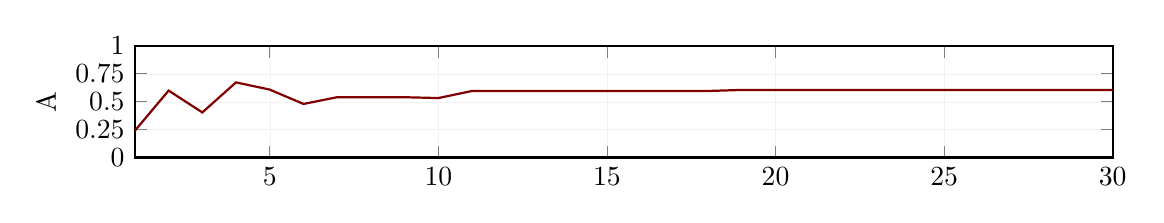
\begin{tikzpicture}
	\begin{axis}[
	yticklabel style={/pgf/number format/fixed},	
	ylabel={A},
	xmin=1, xmax=30,
	ymin=0, ymax=1,
	grid=both,
	grid style={line width=.1pt, draw=gray!10},
	width=14cm,height=3cm,
	xtick={0,5,10,15,20,25,30},
	ytick={0,0.25,0.5,0.75,1},
	thick]
	\addplot[color=Maroon]
	coordinates {
(1,0.239722714509270)(2,0.599103518259375)(3,0.403620935467903)(4,0.672644134189034)(5,0.607817620647413)(6,0.479584136270727)(7,0.539718150016207)(8,0.539718150016207)(9,0.539718150016207)(10,0.532221807225624)(11,0.595551456138064)(12,0.595551456138064)(13,0.595551456138064)(14,0.595551456138064)(15,0.595551456138064)(16,0.595551456138064)(17,0.595551456138064)(18,0.595551456138064)(19,0.604928439081102)(20,0.604928439081102)(21,0.604928439081102)(22,0.604928439081102)(23,0.604928439081102)(24,0.604928439081102)(25,0.604928439081102)(26,0.604928439081102)(27,0.604928439081102)(28,0.604928439081102)(29,0.604928439081102)(30,0.604928439081102)
	};
	\end{axis}
	\end{tikzpicture}
	
	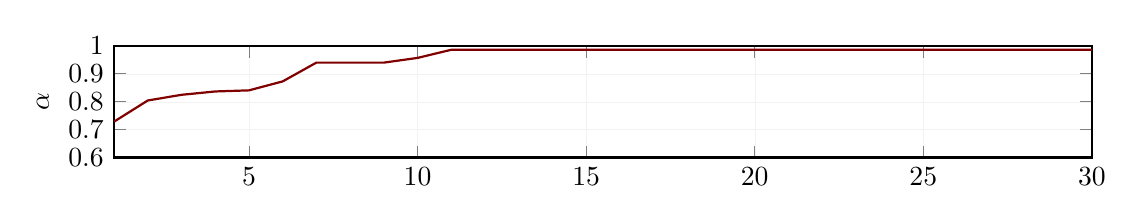
\begin{tikzpicture}
	\begin{axis}[
	yticklabel style={/pgf/number format/fixed},
	ylabel={$\alpha$},
	xmin=1, xmax=30,
	ymin=0.6, ymax=1,
	grid=both,
	grid style={line width=.1pt, draw=gray!10},
	width=14cm,height=3cm,
	xtick={0,5,10,15,20,25,30},
	ytick={0.6,0.7,0.8,0.9,1},
	thick
	]
	
	\addplot[
	color=Maroon
	]
	coordinates {
(1,0.728429668670103)(2,0.804203210919767)(3,0.824520958758779)(4,0.836505338012587)(5,0.840442019998904)(6,0.872518265507127)(7,0.939793685293131)(8,0.939793685293131)(9,0.939793685293131)(10,0.956674409272461)(11,0.985802469943453)(12,0.985802469943453)(13,0.985802469943453)(14,0.985802469943453)(15,0.985802469943453)(16,0.985802469943453)(17,0.985802469943453)(18,0.985802469943453)(19,0.986133844999196)(20,0.986133844999196)(21,0.986133844999196)(22,0.986133844999196)(23,0.986133844999196)(24,0.986133844999196)(25,0.986133844999196)(26,0.986133844999196)(27,0.986133844999196)(28,0.986133844999196)(29,0.986133844999196)(30,0.986133844999196)
	};
	
	\end{axis}
	\end{tikzpicture}
	
	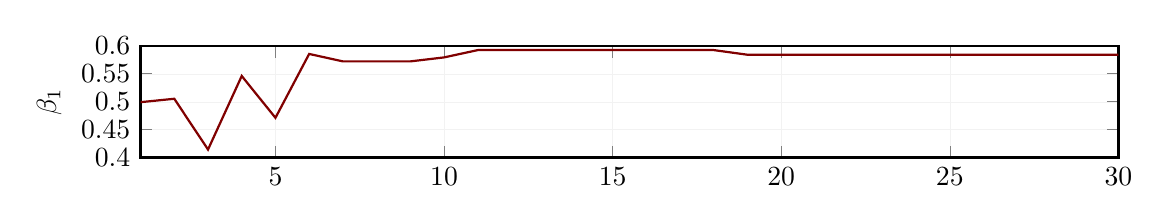
\begin{tikzpicture}
	\begin{axis}[
	yticklabel style={/pgf/number format/fixed},
	ylabel={$\beta_1$},
	xmin=1, xmax=30,
	ymin=0.4, ymax=0.6,
	grid=both,
	grid style={line width=.1pt, draw=gray!10},
	width=14cm,height=3cm,
	xtick={0,5,10,15,20,25,30},
	ytick={0.4,0.45,0.5,0.55,0.6},
	thick
	]
	
	\addplot[color=Maroon]
	coordinates {
(1,0.499080976842225)(2,0.505180603765873)(3,0.414271520778804)(4,0.545954475722939)(5,0.471078169481341)(6,0.585451025200808)(7,0.572105147716796)(8,0.572105147716796)(9,0.572105147716796)(10,0.579243573278727)(11,0.592328138012960)(12,0.592328138012960)(13,0.592328138012960)(14,0.592328138012960)(15,0.592328138012960)(16,0.592328138012960)(17,0.592328138012960)(18,0.592328138012960)(19,0.584016355649755)(20,0.584016355649755)(21,0.584016355649755)(22,0.584016355649755)(23,0.584016355649755)(24,0.584016355649755)(25,0.584016355649755)(26,0.584016355649755)(27,0.584016355649755)(28,0.584016355649755)(29,0.584016355649755)(30,0.584016355649755)
	};
	\end{axis}
	\end{tikzpicture}
	
	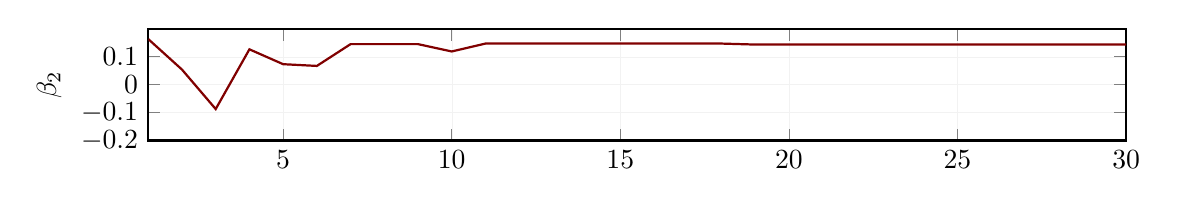
\begin{tikzpicture}
	\begin{axis}[
	yticklabel style={/pgf/number format/fixed},
	ylabel={$\beta_2$},
	xmin=1, xmax=30,
	ymin=-0.2, ymax=0.2,
	grid=both,	      
	scaled y ticks = false,		
	grid style={line width=.1pt, draw=gray!10},
	width=14cm,height=3cm,
	xtick={0,5,10,15,20,25,30},
	ytick={-0.2,-0.1,0,0.1,0.52},
	thick
	]
	
	\addplot[color=Maroon]
	coordinates {
(1,0.163129713702679)(2,0.0538695700526970)(3,-0.0875140579124499)(4,0.126393982708388)(5,0.0731785392834269)(6,0.0669414706805447)(7,0.145001221050750)(8,0.145001221050750)(9,0.145001221050750)(10,0.118718642850213)(11,0.147010707303103)(12,0.147010707303103)(13,0.147010707303103)(14,0.147010707303103)(15,0.147010707303103)(16,0.147010707303103)(17,0.147010707303103)(18,0.147010707303103)(19,0.143471308481112)(20,0.143471308481112)(21,0.143471308481112)(22,0.143471308481112)(23,0.143471308481112)(24,0.143471308481112)(25,0.143471308481112)(26,0.143471308481112)(27,0.143471308481112)(28,0.143471308481112)(29,0.143471308481112)(30,0.143471308481112)
	};
	\end{axis}
	\end{tikzpicture}
	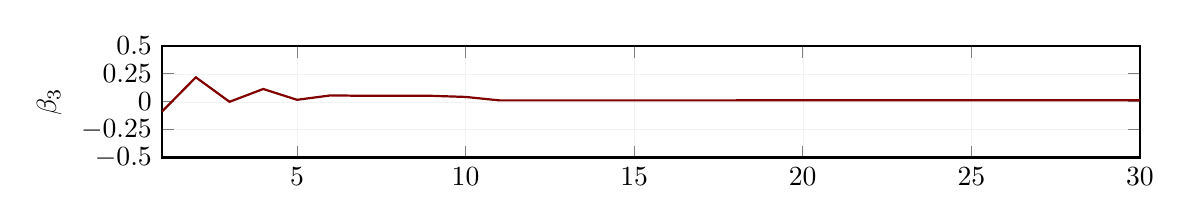
\begin{tikzpicture}
	\begin{axis}[
	yticklabel style={/pgf/number format/fixed},
	ylabel={$\beta_3$},
	xmin=1, xmax=30,
	ymin=-0.5, ymax=0.5,
	grid=both,	      
	scaled y ticks = false,		
	grid style={line width=.1pt, draw=gray!10},
	width=14cm,height=3cm,
	xtick={0,5,10,15,20,25,30},
	ytick={-0.5,-0.25,0,0.25,0.5},
	thick
	]
	
	\addplot[color=Maroon]
	coordinates {
(1,-0.0879647987047510)(2,0.218181685539358)(3,-0.00134177019226656)(4,0.113336425134232)(5,0.0165710539719599)(6,0.0561679929303269)(7,0.0521763755466545)(8,0.0521763755466545)(9,0.0521763755466545)(10,0.0422489067692850)(11,0.0115929080019365)(12,0.0115929080019365)(13,0.0115929080019365)(14,0.0115929080019365)(15,0.0115929080019365)(16,0.0115929080019365)(17,0.0115929080019365)(18,0.0115929080019365)(19,0.0134068930918946)(20,0.0134068930918946)(21,0.0134068930918946)(22,0.0134068930918946)(23,0.0134068930918946)(24,0.0134068930918946)(25,0.0134068930918946)(26,0.0134068930918946)(27,0.0134068930918946)(28,0.0134068930918946)(29,0.0134068930918946)(30,0.0134068930918946)
	};
	\end{axis}
	\end{tikzpicture}
	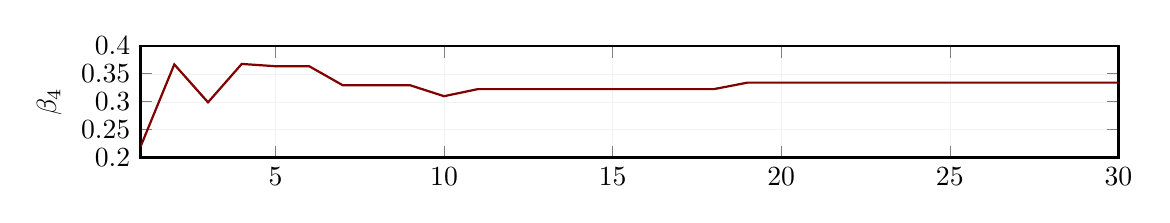
\begin{tikzpicture}
	\begin{axis}[
	yticklabel style={/pgf/number format/fixed},
	ylabel={$\beta_4$},
	xmin=1, xmax=30,
	ymin=0.2, ymax=0.4,
	grid=both,	      
	scaled y ticks = false,		
	grid style={line width=.1pt, draw=gray!10},
	width=14cm,height=3cm,
	xtick={0,5,10,15,20,25,30},
	ytick={0.2,0.25,0.3,0.35,0.4},
	thick
	]
	
	\addplot[color=Maroon]
	coordinates {
(1,0.219602483845886)(2,0.366697231160561)(3,0.298787535003235)(4,0.367545304095982)(5,0.363450227067740)(6,0.363454605113127)(7,0.329262060005046)(8,0.329262060005046)(9,0.329262060005046)(10,0.309802533862957)(11,0.322418967762391)(12,0.322418967762391)(13,0.322418967762391)(14,0.322418967762391)(15,0.322418967762391)(16,0.322418967762391)(17,0.322418967762391)(18,0.322418967762391)(19,0.334083300066931)(20,0.334083300066931)(21,0.334083300066931)(22,0.334083300066931)(23,0.334083300066931)(24,0.334083300066931)(25,0.334083300066931)(26,0.334083300066931)(27,0.334083300066931)(28,0.334083300066931)(29,0.334083300066931)(30,0.334083300066931)
	};
	\end{axis}
	\end{tikzpicture}
	\begin{tikzpicture}
	\begin{axis}[
	yticklabel style={/pgf/number format/fixed},
	ylabel={$\beta_5$},
	xmin=1, xmax=30,
	ymin=-0.2, ymax=0.2,
	grid=both,	      
	scaled y ticks = false,		
	grid style={line width=.1pt, draw=gray!10},
	width=14cm,height=3cm,
	xtick={0,5,10,15,20,25,30},
	ytick={-0.2,-0.1,0,0.1,0.2},
	thick
	]
	
	\addplot[color=Maroon]
	coordinates {
(1,-0.0143745560760625)(2,0.0704098188011883)(3,-0.0435970414999130)(4,0.00163969132816741)(5,-0.168350654551373)(6,0.0748959275178980)(7,0.0864157946524996)(8,0.0864157946524996)(9,0.0864157946524996)(10,0.0632604024743052)(11,0.0473459847516897)(12,0.0473459847516897)(13,0.0473459847516897)(14,0.0473459847516897)(15,0.0473459847516897)(16,0.0473459847516897)(17,0.0473459847516897)(18,0.0473459847516897)(19,0.0405385305601807)(20,0.0405385305601807)(21,0.0405385305601807)(22,0.0405385305601807)(23,0.0405385305601807)(24,0.0405385305601807)(25,0.0405385305601807)(26,0.0405385305601807)(27,0.0405385305601807)(28,0.0405385305601807)(29,0.0405385305601807)(30,0.0405385305601807)
	};
	\end{axis}
	\end{tikzpicture}
	\begin{tikzpicture}
	\begin{axis}[
	yticklabel style={/pgf/number format/fixed},
	xlabel={Generation},
	ylabel={$\beta_6$},
	xmin=1, xmax=30,
	ymin=-0.5, ymax=0.5,
	grid=both,	      
	scaled y ticks = false,		
	grid style={line width=.1pt, draw=gray!10},
	width=14cm,height=3cm,
	xtick={0,5,10,15,20,25,30},
	ytick={-0.5,0.25,0,0.25,0.5},
	thick
	]
	
	\addplot[color=Maroon]
	coordinates {
(1,-0.0408684911700100)(2,0.288338955700592)(3,0.119379290581781)(4,0.359907497802918)(5,0.256628407789643)(6,0.492299086893167)(7,0.442698042043135)(8,0.442698042043135)(9,0.442698042043135)(10,0.460196090920927)(11,0.486763275977465)(12,0.486763275977465)(13,0.486763275977465)(14,0.486763275977465)(15,0.486763275977465)(16,0.486763275977465)(17,0.486763275977465)(18,0.486763275977465)(19,0.492414778303015)(20,0.492414778303015)(21,0.492414778303015)(22,0.492414778303015)(23,0.492414778303015)(24,0.492414778303015)(25,0.492414778303015)(26,0.492414778303015)(27,0.492414778303015)(28,0.492414778303015)(29,0.492414778303015)(30,0.492414778303015)
	};
	\end{axis}
	\end{tikzpicture}
	\caption{Modified Firefly Algorithm -- Generalized Bouc-Wen Model}
	\label{fig:mfa_gen_trend}
\end{figure}

The final values found for each parameter using the Modified Firefly Algorithm approach
are displayed in Table~\ref{tab:mfa_gen_values}.

\begin{table}[H]
	\centering
	\begin{tabular}{l c c c c c c c c}
		\toprule
		\textbf{Parameter}		& $A$		& $\alpha$	& $\beta_1$	& $\beta_2$ & $\beta_3$	& $\beta_4$ & $\beta_5$ & $\beta_6$		\\ \midrule
		\textbf{Final value}	& $0.6049$	& $0.9861$	& $0.5840$ & $0.1435$ & $0.0134$	& $0.3341$	& $0.0405$	& $0.4924$	\\
		\bottomrule
	\end{tabular}
	\caption{Modified Firefly Algorithm -- Final values (Generalized Bouc-Wen model)}
	\label{tab:mfa_gen_values}
\end{table}

\subsubsection{Particle Swarm Optimization -- Generalized Bouc-Wen Model}

Table~\ref{tab:pso_gen_params} contains the parameters used for the
Particle Swarm Optimization approach.
The hysteresis loop behaviour with the final parameters is displayed
in Figure~\ref{fig:pso_gen_final}.
Figure~\ref{fig:pso_gen_trend} shows the trend of generalized Bouc-Wen model parameters
using the Particle Swarm Optimization approach.

\begin{table}[H]
	\centering
	\begin{tabular}{c c}
		\toprule
		\textbf{Parameter} & \textbf{Value} \\ \toprule
		$N$			& $10$ \\
		$G$			& $30$ \\
		$d$			& $8$  \\
		$L$			& $\left[0, 0, -0.1, -0.1, -0.1, -0.1, -0.1, -0.1\right]$ \\
		$U$			& $\left[2, 0.9, 1, 1, 1, 1, 1, 1 \right]$ \\ 
		$a$			& $2.1$ \\
		$b$			& $0.6$ \\ 
		$c_1$		& $2$	\\
		$c_2$		& $2$	\\ 
		$V_{max}$	& $\left[0.1,0.1,0.1,0.1,0.1,0.1,0.1,0.1\right]$ \\ \bottomrule
	\end{tabular}
	\caption{Parameters for the Particle Swarm Optimization approach -- Generalized Bouc-Wen model}
	\label{tab:pso_gen_params}
\end{table}

\begin{figure}[H]
	\centering
	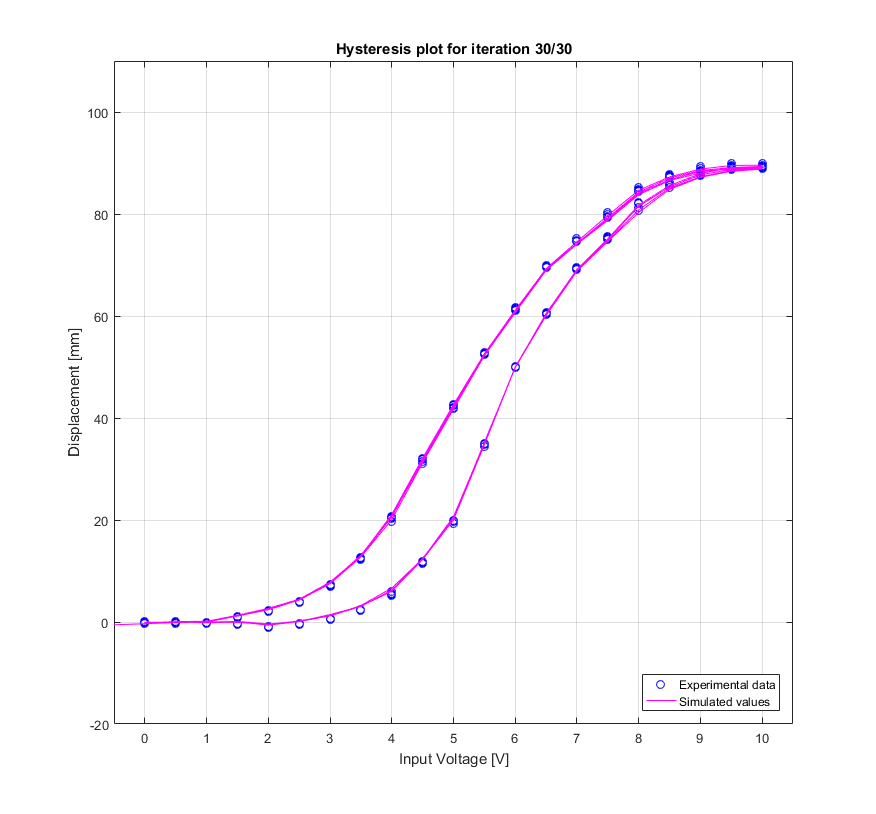
\includegraphics[width=0.85\linewidth]{Images/pso_gen_final}
	\caption{Hysteresis loop result using Particle Swarm Optimization parameters (generalized Bouc-Wen model)}
	\label{fig:pso_gen_final}
\end{figure}

\begin{figure}[H]
	\centering
	\begin{tikzpicture}
	\begin{axis}[
	yticklabel style={/pgf/number format/fixed},	
	ylabel={A},
	xmin=1, xmax=30,
	ymin=1.6, ymax=2,
	grid=both,
	grid style={line width=.1pt, draw=gray!10},
	width=14cm,height=3cm,
	xtick={0,5,10,15,20,25,30},
	ytick={1.6,1.7,1.8,1.9,2},
	thick]
	\addplot[color=Maroon]
	coordinates {
(1,1.79761151203321)(2,2)(3,1.87111132774023)(4,1.87111132774023)(5,1.87111132774023)(6,1.87111132774023)(7,1.87111132774023)(8,1.87111132774023)(9,1.87111132774023)(10,1.87111132774023)(11,1.87111132774023)(12,1.87111132774023)(13,1.87111132774023)(14,1.87111132774023)(15,1.87111132774023)(16,2)(17,2)(18,2)(19,2)(20,2)(21,2)(22,2)(23,2)(24,2)(25,2)(26,2)(27,2)(28,2)(29,2)(30,2)
	};
	\end{axis}
	\end{tikzpicture}
	
	\begin{tikzpicture}
	\begin{axis}[
	yticklabel style={/pgf/number format/fixed},
	ylabel={$\alpha$},
	xmin=1, xmax=30,
	ymin=0.6, ymax=1,
	grid=both,
	grid style={line width=.1pt, draw=gray!10},
	width=14cm,height=3cm,
	xtick={0,5,10,15,20,25,30},
	ytick={0.6,0.7,0.8,0.9,1},
	thick
	]
	
	\addplot[
	color=Maroon
	]
	coordinates {
(1,0.759865547111675)(2,0.680147815008967)(3,0.990000000000000)(4,0.990000000000000)(5,0.990000000000000)(6,0.990000000000000)(7,0.990000000000000)(8,0.990000000000000)(9,0.990000000000000)(10,0.990000000000000)(11,0.990000000000000)(12,0.990000000000000)(13,0.990000000000000)(14,0.990000000000000)(15,0.990000000000000)(16,0.990000000000000)(17,0.990000000000000)(18,0.990000000000000)(19,0.990000000000000)(20,0.990000000000000)(21,0.990000000000000)(22,0.990000000000000)(23,0.990000000000000)(24,0.990000000000000)(25,0.990000000000000)(26,0.990000000000000)(27,0.990000000000000)(28,0.990000000000000)(29,0.990000000000000)(30,0.990000000000000)
	};
	
	\end{axis}
	\end{tikzpicture}
	
	\begin{tikzpicture}
	\begin{axis}[
	yticklabel style={/pgf/number format/fixed},
	ylabel={$\beta_1$},
	xmin=1, xmax=30,
	ymin=0, ymax=0.5,
	grid=both,
	grid style={line width=.1pt, draw=gray!10},
	width=14cm,height=3cm,
	xtick={0,5,10,15,20,25,30},
	ytick={0,0.125,0.25,0.375,0.5},
	thick
	]
	
	\addplot[color=Maroon]
	coordinates {
(1,0.163612892901600)(2,0.317489418613579)(3,0.456236491818980)(4,0.456236491818980)(5,0.456236491818980)(6,0.456236491818980)(7,0.456236491818980)(8,0.456236491818980)(9,0.456236491818980)(10,0.456236491818980)(11,0.456236491818980)(12,0.456236491818980)(13,0.456236491818980)(14,0.456236491818980)(15,0.456236491818980)(16,0.366897198955879)(17,0.366897198955879)(18,0.366897198955879)(19,0.366897198955879)(20,0.366897198955879)(21,0.366897198955879)(22,0.366897198955879)(23,0.366897198955879)(24,0.366897198955879)(25,0.366897198955879)(26,0.366897198955879)(27,0.366897198955879)(28,0.366897198955879)(29,0.366897198955879)(30,0.309562322949807)
	};
	\end{axis}
	\end{tikzpicture}
	
	\begin{tikzpicture}
	\begin{axis}[
	yticklabel style={/pgf/number format/fixed},
	ylabel={$\beta_2$},
	xmin=1, xmax=30,
	ymin=-0.2, ymax=0.2,
	grid=both,	      
	scaled y ticks = false,		
	grid style={line width=.1pt, draw=gray!10},
	width=14cm,height=3cm,
	xtick={0,5,10,15,20,25,30},
	ytick={-0.2,-0.1,0,0.1,0.52},
	thick
	]
	
	\addplot[color=Maroon]
	coordinates {
(1,0.164455554793160)(2,-0.100000000000000)(3,-0.100000000000000)(4,-0.100000000000000)(5,-0.100000000000000)(6,-0.100000000000000)(7,-0.100000000000000)(8,-0.100000000000000)(9,-0.100000000000000)(10,-0.100000000000000)(11,-0.100000000000000)(12,-0.100000000000000)(13,-0.100000000000000)(14,-0.100000000000000)(15,-0.100000000000000)(16,-0.100000000000000)(17,-0.100000000000000)(18,-0.100000000000000)(19,-0.100000000000000)(20,-0.100000000000000)(21,-0.100000000000000)(22,-0.100000000000000)(23,-0.100000000000000)(24,-0.100000000000000)(25,-0.100000000000000)(26,-0.100000000000000)(27,-0.100000000000000)(28,-0.100000000000000)(29,-0.100000000000000)(30,-0.100000000000000)
	};
	\end{axis}
	\end{tikzpicture}
	\begin{tikzpicture}
	\begin{axis}[
	yticklabel style={/pgf/number format/fixed},
	ylabel={$\beta_3$},
	xmin=1, xmax=30,
	ymin=-0.5, ymax=0.5,
	grid=both,	      
	scaled y ticks = false,		
	grid style={line width=.1pt, draw=gray!10},
	width=14cm,height=3cm,
	xtick={0,5,10,15,20,25,30},
	ytick={-0.5,-0.25,0,0.25,0.5},
	thick
	]
	
	\addplot[color=Maroon]
	coordinates {
(1,0.220984156136484)(2,-0.100000000000000)(3,-0.100000000000000)(4,-0.100000000000000)(5,-0.100000000000000)(6,-0.100000000000000)(7,-0.100000000000000)(8,-0.100000000000000)(9,-0.100000000000000)(10,-0.100000000000000)(11,-0.100000000000000)(12,-0.100000000000000)(13,-0.100000000000000)(14,-0.100000000000000)(15,-0.100000000000000)(16,-0.100000000000000)(17,-0.100000000000000)(18,-0.100000000000000)(19,-0.100000000000000)(20,-0.100000000000000)(21,-0.100000000000000)(22,-0.100000000000000)(23,-0.100000000000000)(24,-0.100000000000000)(25,-0.100000000000000)(26,-0.100000000000000)(27,-0.100000000000000)(28,-0.100000000000000)(29,-0.100000000000000)(30,-0.100000000000000)
	};
	\end{axis}
	\end{tikzpicture}
	\begin{tikzpicture}
	\begin{axis}[
	yticklabel style={/pgf/number format/fixed},
	ylabel={$\beta_4$},
	xmin=1, xmax=30,
	ymin=-0.1, ymax=0.1,
	grid=both,	      
	scaled y ticks = false,		
	grid style={line width=.1pt, draw=gray!10},
	width=14cm,height=3cm,
	xtick={0,5,10,15,20,25,30},
	ytick={-0.1,-0.05,0,0.05,0.1},
	thick
	]
	
	\addplot[color=Maroon]
	coordinates {
(1,0.0382242187526582)(2,-0.100000000000000)(3,-0.100000000000000)(4,-0.100000000000000)(5,-0.100000000000000)(6,-0.100000000000000)(7,-0.100000000000000)(8,-0.100000000000000)(9,-0.100000000000000)(10,-0.100000000000000)(11,-0.100000000000000)(12,-0.100000000000000)(13,-0.100000000000000)(14,-0.100000000000000)(15,-0.100000000000000)(16,-0.100000000000000)(17,-0.100000000000000)(18,-0.100000000000000)(19,-0.100000000000000)(20,-0.100000000000000)(21,-0.100000000000000)(22,-0.100000000000000)(23,-0.100000000000000)(24,-0.100000000000000)(25,-0.100000000000000)(26,-0.100000000000000)(27,-0.100000000000000)(28,-0.100000000000000)(29,-0.100000000000000)(30,-0.100000000000000)
	};
	\end{axis}
	\end{tikzpicture}
	\begin{tikzpicture}
	\begin{axis}[
	yticklabel style={/pgf/number format/fixed},
	ylabel={$\beta_5$},
	xmin=1, xmax=30,
	ymin=0.8, ymax=1,
	grid=both,	      
	scaled y ticks = false,		
	grid style={line width=.1pt, draw=gray!10},
	width=14cm,height=3cm,
	xtick={0,5,10,15,20,25,30},
	ytick={0.8,-0.85,0.9,0.95,1},
	thick
	]
	
	\addplot[color=Maroon]
	coordinates {
(1,0.857797418753933)(2,0.883110501479002)(3,1)(4,1)(5,1)(6,1)(7,1)(8,1)(9,1)(10,1)(11,1)(12,1)(13,1)(14,1)(15,1)(16,1)(17,1)(18,1)(19,1)(20,1)(21,1)(22,1)(23,1)(24,1)(25,1)(26,1)(27,1)(28,1)(29,1)(30,1)
	};
	\end{axis}
	\end{tikzpicture}
	\begin{tikzpicture}
	\begin{axis}[
	yticklabel style={/pgf/number format/fixed},
	xlabel={Generation},
	ylabel={$\beta_6$},
	xmin=1, xmax=30,
	ymin=0.5, ymax=1,
	grid=both,	      
	scaled y ticks = false,		
	grid style={line width=.1pt, draw=gray!10},
	width=14cm,height=3cm,
	xtick={0,5,10,15,20,25,30},
	ytick={0.5,0.625,0.75,0.875,1},
	thick
	]
	
	\addplot[color=Maroon]
	coordinates {
(1,0.919048321968003)(2,1)(3,0.571300777361267)(4,0.571300777361267)(5,0.571300777361267)(6,0.571300777361267)(7,0.571300777361267)(8,0.571300777361267)(9,0.571300777361267)(10,0.571300777361267)(11,0.571300777361267)(12,0.571300777361267)(13,0.571300777361267)(14,0.571300777361267)(15,0.571300777361267)(16,0.561660614151037)(17,0.561660614151037)(18,0.561660614151037)(19,0.561660614151037)(20,0.561660614151037)(21,0.561660614151037)(22,0.561660614151037)(23,0.561660614151037)(24,0.561660614151037)(25,0.561660614151037)(26,0.561660614151037)(27,0.561660614151037)(28,0.561660614151037)(29,0.561660614151037)(30,0.554539257473428)
	};
	\end{axis}
	\end{tikzpicture}
	\caption{Particle Swarm Optimization -- Generalized Bouc-Wen Model}
	\label{fig:pso_gen_trend}
\end{figure}

The final values found for each parameter using the Particle Swarm Optimization approach
are displayed in Table~\ref{tab:pso_gen_values}.

\begin{table}[H]
	\centering
	\begin{tabular}{l c c c c c c c c}
		\toprule
		\textbf{Parameter}		& $A$		& $\alpha$	& $\beta_1$	& $\beta_2$ & $\beta_3$	& $\beta_4$ & $\beta_5$ & $\beta_6$		\\ \midrule
		\textbf{Final value}	& $2$	& $0.99$	& $0.3096$ & $-0.1$ & $-0.1$	& $-0.1$	& $1$	& $0.5545$	\\
		\bottomrule
	\end{tabular}
	\caption{Particle Swarm Optimization -- Final values (Generalized Bouc-Wen model)}
	\label{tab:pso_gen_values}
\end{table}

\subsection{Time Comparison}
\label{sec:5.comparison_time}

In order to be relevant, timing comparisons among the algorithms previously described
have to be made with the same number of individuals in the population.
This ensures impartiality between them when it comes to ranking the algorithms
for performance.

Each algorithm has been thus ran with a variable number of candidate solutions of
10, 20 and 30, and the total execution time has been recorded.
For each algorithm and each number of candidate solutions,
a average execution time per generation is presented. The intent
is to rank them by execution time and relative precision.

Table~\ref{tab:timing} displays the differences in execution times
for all algorithms with different numbers of individuals in the population.
The number of generations/iterations has been set to 30 for all algorithms.

For the Genetic Algorithm approach, it has been observed that the crossover
strategy chosen does not affect the execution time. For this reason
the values presented in the table refer to execution times obtained
with the proportional crossover method.

\begin{table}[H]
	\centering
	\begin{tabular}{c c c c c c}
		\toprule
		\thead{ Number of \\ individuals}	&	\thead{ Algorithm}	&	\thead{ Total time \\ (Classic)}	& \thead{ Average Time \\ (Classic)}	& \thead{ Total Time \\ (Generalized)} &	\thead{ Average Time \\ (Generalized)}	\\
		\midrule
		10 	& GA	& 21.98 s	& 0.73 s	& 30.72 s	& 1.02 s	\\
			& MFA	& 21.34 s	& 0.71 s	& 30.78 s	& 1.03 s	\\
			& PSO	& 21.36 s	& 0.71 s	& 30.57 s	& 1.02 s	\\ \midrule
		20	& GA	& 37.96 s	& 1.26 s	& 59.65 s	& 1.99 s	\\
			& MFA	& 39.43 s	& 1.31 s	& 60.36 s	& 2.01 s	\\
			& PSO	& 40.84 s	& 1.36 s	& 62.79 s	& 2.09 s	\\ \midrule
		30	& GA	& 55.45 s	& 1.85 s	& 84.18 s	& 2.81 s	\\
			& MFA	& 54.32 s	& 1.81 s	& 85.04 s	& 2.83 s	\\
			& PSO	& 55.40 s	& 1.84 s	& 82.31 s	& 2.74 s	\\ \bottomrule
	\end{tabular}
\caption{Timing performance comparison among algorithms}
\label{tab:timing}
\end{table}

Timing results of Table~\ref{tab:timing} must be compared also to the relative
precision of the final solution proposed by each algorithm: as a matter of fact,
in the case of the Genetic Algorithm method, a lower number of individuals 
in the population brings timing results almost identical to those of the other two
algorithms, but the precision heavily depend on the chromosomes of individuals
that are generated initially. In the other two algorithms, the global exploration
approach undertaken by the fireflies/particles make them wander faster across
the solution space. Therefore, the lower number of individuals does not
cause a lower precision as much.

The timing performance of the three algorithms make them not suitable for online control.
There may be an improvement in performance if the algorithms were implemented onto
dedicated hardware, e.g. a single purpose processor or a video card programmed
to faster calculate the evolution of individuals, or the movement of fireflies/particles.



